% =====================================================================
%  ESTRUCTURA DEL DOCUMENTO ERS/SRS -- ENTREGA 2 (1B)
%  Ingenieria de Requerimientos [20303] -- UTEQ -- 2026-2027 PPA
% =====================================================================
\documentclass[11pt,a4paper]{article}
\usepackage[utf8]{inputenc}
\usepackage[T1]{fontenc}
\usepackage{times}
\usepackage{amssymb}
\renewcommand{\familydefault}{\rmdefault}

\usepackage[a4paper, top=3cm, bottom=2.5cm, left=2.5cm, right=2.5cm]{geometry}
\usepackage[table]{xcolor}
\definecolor{uteqgreen}{HTML}{1D6B36}
\definecolor{uteqgold}{HTML}{D4A017}
\definecolor{uteqblue}{HTML}{1A5276}
\definecolor{secdark}{HTML}{1A3A6B}
\definecolor{lightgray}{HTML}{F5F5F5}

\usepackage{array}
\usepackage{tabularx}
\usepackage{enumitem}
\usepackage{graphicx}
\usepackage{microtype}
\usepackage{parskip}
\usepackage{fancyhdr}
\usepackage{lastpage}
\usepackage[bookmarksnumbered]{hyperref}
\hypersetup{
    colorlinks=true,
    linkcolor=uteqblue,
    urlcolor=uteqgreen,
    pdftitle={ERS/SRS - Entrega 2 (1B)}
}

\setlist{leftmargin=1.5em, topsep=2pt, itemsep=1pt}

\pagestyle{fancy}
\fancyhf{}
\renewcommand{\headrulewidth}{0.4pt}
\renewcommand{\footrulewidth}{0.4pt}
\fancyhead[L]{\textbf{\color{black}ERS/SRS}}
\fancyhead[R]{\color{uteqgold}Entrega 2 (1B)}
\fancyfoot[C]{\thepage}

% =====================================================================
%  COMANDOS PARA SECCIONES (CON ÍNDICE Y JUSTIFICACIÓN)
% =====================================================================

\newcounter{secc}
\newcommand{\secband}[1]{%
    \stepcounter{secc}%
    \phantomsection%
    \addcontentsline{toc}{section}{\protect\numberline{\arabic{secc}}#1}%
    \par\vspace{12pt}\noindent
    {\setlength{\fboxsep}{0pt}%
    \colorbox{uteqgold}{\parbox[c][22pt][c]{0.06\textwidth}{\centering\textbf{\color{white}\large \arabic{secc}}}}%
    \colorbox{uteqgreen}{\parbox[c][22pt][c]{0.94\textwidth}{\hspace{10pt}\textbf{\color{white}\large #1}}}%
    }\par\vspace{8pt}}

\newcounter{slinecounter}[secc]
\renewcommand{\theslinecounter}{\arabic{secc}.\arabic{slinecounter}}
\newcommand{\sline}[1]{%
    \stepcounter{slinecounter}%
    \addcontentsline{toc}{subsection}{\protect\numberline{\theslinecounter}#1}%
    \par\vspace{6pt}\noindent
    \textbf{\color{uteqgreen}\large \theslinecounter\quad #1}\par\vspace{4pt}}

\newcounter{sslinecounter}[slinecounter]
\renewcommand{\thesslinecounter}{\arabic{secc}.\arabic{slinecounter}.\arabic{sslinecounter}}
\newcommand{\ssline}[1]{%
    \stepcounter{sslinecounter}%
    \addcontentsline{toc}{subsubsection}{\protect\numberline{\thesslinecounter}#1}%
    \par\noindent
    \textbf{\color{uteqblue}\thesslinecounter\quad #1}\par\vspace{2pt}}

% =====================================================================
%  INICIO DEL DOCUMENTO
% =====================================================================

\begin{document}

% =====================================================================
%  PORTADA
% =====================================================================

\begin{center}
    \vspace*{1cm}
    {\large\bfseries\color{secdark}FACULTAD DE CIENCIAS DE LA COMPUTACIÓN}\\[4pt]
    {\large\bfseries\color{secdark}INGENIERÍA DE REQUERIMIENTOS [20303]}\\[4pt]
    {\large\bfseries\color{secdark}PROYECTO FIN DE CURSO}\\[8pt]
    \textcolor{uteqgold}{\rule{0.6\textwidth}{2pt}}\\[12pt]
    {\Huge\bfseries\color{black}Sistema de Movilidad Colaborativa para la Comunidad Universitaria de la UTEQ}\\[4pt]
    {\Large\bfseries\color{uteqgold}(ERS/SRS)}\\[12pt]
    \textcolor{uteqgold}{\rule{0.6\textwidth}{1pt}}\\[10pt]
    {\Large\bfseries\color{black}ENTREGA 2 (1B)}\\[8pt]
    \textcolor{white}{\rule{0.6\textwidth}{1pt}}\\[10pt]
    
\includegraphics[width=0.15\textwidth]{UTEQ LOGO.png}\\[25pt]
    {\large\bfseries\color{secdark}Equipo de Trabajo:}\\[2pt]
    {\large Cordova Carreño Mayra Lucila - Diseñadora de Modelos}\\[2pt]
    {\large Herrera Moran Gilmar Javier - Analista de Requerimientos}\\[2pt]
    {\large Naranjo Flores Anderson Jeampiere - Analista Líder / Gestión de Proyecto}\\[2pt]
    {\large Valarezo Flores Steven Alexander - Analista de Requerimientos / Investigador de Campo}\\[8pt]
    {\large\bfseries\color{secdark}Docente:} {\large Phd. Guerrero Ulloa Gleiston Ciceron}\\[4pt]
    {\large\bfseries\color{secdark}Fecha:} {\large \today}\\[4pt]
    {\large\bfseries\color{secdark}Versión:} {\large 2.0}\\[8pt]
    {\large\bfseries\color{uteqblue}Repositorio:} {\large \url{https://github.com/AnderJM3/IngReq-B-2026-PPA}}\\[4pt]
    \textcolor{uteqgold}{\rule{0.4\textwidth}{1pt}}\\[10pt]
    {\small \color{black}PPA 2026-2027}\\
    {\small \color{black}Quevedo - Ecuador}
\end{center}

\newpage

% =====================================================================
%  HISTORIAL DE VERSIONES
% =====================================================================

\section*{HISTORIAL DE VERSIONES}

\begin{tabularx}{\textwidth}{|c|c|c|X|}
\hline
\textbf{Versión} & \textbf{Fecha} & \textbf{Autor} & \textbf{Descripción del cambio} \\
\hline
0.1 & 28/06/2026 & Equipo CMVZ & Creación inicial del documento ERS/SRS \\
\hline
0.5 & 28/06/2026 & Equipo CMVZ & Integración de requisitos, interfaces y mockups \\
\hline
0.8 & 28/06/2026 & Equipo CMVZ & Inclusión de UML, MoSCoW y trazabilidad \\
\hline
1.0 & 28/06/2026 & Equipo CMVZ & Primera versión consolidada de Entrega 1B \\
\hline
1.1 & 30/06/2026 & Equipo CMVZ & Corrección de portada, evidencias, multimedia, consentimientos, GitHub y trazabilidad \\
\hline
\end{tabularx}

\newpage

% =====================================================================
%  TABLA DE CONTENIDO
% =====================================================================

\tableofcontents
\newpage
\listoffigures
\newpage
\listoftables
\newpage

% =====================================================================
%  1. INTRODUCCIÓN
% =====================================================================

\secband{INTRODUCCIÓN}

\sline{Propósito del documento}

El presente documento corresponde a la Entrega 1B de la Especificación de Requisitos de Software (ERS/SRS) del \textbf{Sistema de Movilidad Colaborativa para la Comunidad Universitaria de la UTEQ}. Su elaboración toma como base la información obtenida y corregida en la Entrega 1A y sigue una estructura tipo IEEE/ISO/IEC 29148 para la especificación de requisitos de software. Este documento servirá como guía para las etapas de diseño, desarrollo, validación y trazabilidad del sistema.

El Sistema de Movilidad Colaborativa surge como una respuesta a las dificultades que enfrentan actualmente los estudiantes y docentes de la UTEQ para trasladarse hacia los campus Central y La María. Esta problemática se ve agravada por factores como la distancia, los costos de transporte y la falta de alternativas sostenibles. Ante este escenario, el sistema se propone como una solución tecnológica que utiliza inteligencia artificial y análisis de datos para facilitar el transporte compartido y optimizar la movilidad universitaria.

\sline{Alcance del producto}

\begin{table}[h]
    \centering
    \caption{Alcance del producto}
    \label{tab:alcance}
    \vspace{6pt}
    \begin{tabularx}{\textwidth}{|l|X|}
    \hline
    \textbf{Incluido} & \textbf{Excluido} \\
    \hline
    Registro y validación de usuarios mediante credenciales institucionales & Diagnóstico de problemas de movilidad fuera del ámbito universitario \\
    \hline
    Publicación, búsqueda y coordinación de rutas de transporte compartido & Atención de emergencias médicas o de seguridad vial \\
    \hline
    Recomendación automática de rutas mediante inteligencia artificial & Gestión de flotas de vehículos institucionales \\
    \hline
    Gestión de perfiles y atención de incidencias operativas & Sistema de pago o transacciones monetarias \\
    \hline
    Generación de reportes y estadísticas para la administración & Integración con sistemas de transporte público externos \\
    \hline
    Análisis de patrones de movilidad e identificación de horarios con alta demanda & Sustitución de la planificación de transporte institucional \\
    \hline
    \end{tabularx}
\end{table}

\sline{Definiciones, acrónimos y abreviaturas}

\begin{tabularx}{\textwidth}{|l|X|}
\hline
\textbf{Término} & \textbf{Definición} \\
\hline
Carpooling & Sistema de transporte compartido donde varios usuarios comparten un vehículo para realizar un trayecto común \\
\hline
Movilidad colaborativa & Modelo de transporte basado en la cooperación entre usuarios para optimizar desplazamientos \\
\hline
Ruta & Trayecto definido por un origen, destino, horario y cupos disponibles \\
\hline
Conductor universitario & Miembro de la comunidad UTEQ que ofrece transporte compartido en su vehículo \\
\hline
Pasajero & Usuario que solicita un viaje compartido \\
\hline
Algoritmo de recomendación & Sistema de IA que sugiere rutas compatibles según el historial y preferencias del usuario \\
\hline
Geolocalización & Tecnología que permite determinar la posición geográfica de un dispositivo \\
\hline
\end{tabularx}

\sline{Referencias}

[1] S. AlQuhtani, ``Ridesharing as a Potential Sustainable Transportation Alternative in Suburban Universities: The Case of Najran University, Saudi Arabia,'' \textit{Sustainability}, vol. 14, no. 8, p. 4392, 2022.

[2] R. López-Chila, M. Dávila-Moreno, G. Muñoz-Franco, and M. Estrella-Guayasamin, ``Methodology and Innovation in the Design of Shared Transportation Systems for Academic Environments,'' \textit{Sustainability}, vol. 17, 2025.

[3] ISO/IEC, \textit{ISO/IEC/IEEE 29148:2018: Systems and software engineering -- Life cycle processes -- Requirements engineering}. ISO, 2018.

[4] Pressman, R. S. \textit{Software Engineering: A Practitioner's Approach}. 8th ed. McGraw-Hill, 2014.

\sline{Visión general del documento}

La presente Especificación de Requisitos de Software (ERS/SRS) se encuentra estructurada de manera lógica y secuencial para facilitar la comprensión integral de las necesidades y capacidades del Sistema de Movilidad Colaborativa para la Comunidad Universitaria de la UTEQ. El documento se organiza en seis capítulos principales que guían al lector desde la descripción general del proyecto hasta la especificación detallada de los requisitos del sistema, pasando por el modelado UML, la priorización y la trazabilidad.

Capítulo 1 este capítulo presenta la introducción el propósito del documento, el alcance del producto, las definiciones, acrónimos y abreviaturas, las referencias utilizadas y la organización general de la especificación. Su objetivo es proporcionar al lector una visión panorámica del proyecto y establecer el contexto necesario para comprender el resto del documento.

Capítulo 2 este capítulo describe la descripción general del sistema, incluyendo la perspectiva del producto, sus funciones principales, las características de los usuarios (perfiles y roles), el mapa de stakeholders, el entorno operativo, las suposiciones y dependencias que influyen en el desarrollo del proyecto. Su objetivo es situar al lector en el entorno del sistema y comprender las condiciones en las que operará.

Capítulo 3 este capítulo presenta la especificación detallada de los requisitos del sistema, incorporando los requisitos funcionales (con su plantilla de 8 atributos), los requisitos no funcionales (cuantificados bajo ISO/IEC 25010), las interfaces externas (usuario, hardware y software) y las restricciones de diseño. Su objetivo es definir de manera formal y verificable todas las funcionalidades y condiciones de calidad que debe cumplir el sistema.

Capítulo 4 este capítulo desarrolla el modelado del sistema mediante diagramas UML, incluyendo el diagrama de casos de uso general, la especificación textual detallada de al menos cinco casos de uso, y el diagrama de clases conceptual. Su objetivo es representar visualmente la estructura y el comportamiento del sistema, facilitando la comunicación entre stakeholders y el equipo de desarrollo.

Capítulo 5 este capítulo presenta la clasificación de requisitos (RF, NFR y restricciones), la priorización mediante la técnica MoSCoW con justificación de cada clasificación, y la matriz de trazabilidad parcial que relaciona evidencias, requisitos y casos de uso. Su objetivo es garantizar que los requisitos sean gestionables, priorizables y trazables a lo largo del ciclo de vida del software.

Capítulo 6 este capítulo resume los logros alcanzados en la entrega, las decisiones de diseño tempranas y el trabajo pendiente para la siguiente fase del proyecto (Entrega 2A). Su objetivo es cerrar el documento con una reflexión sobre el estado del proyecto y los pasos a seguir.

Los apéndices complementan el documento con información detallada sobre: el plan del proyecto de Ingeniería de Requisitos (Apéndice A), el trabajo de campo y evidencias recopiladas (Apéndice B), la clasificación MoSCoW detallada (Apéndice C), la matriz de trazabilidad completa (Apéndice D), y el repositorio GitHub (Apéndice E). Su objetivo es proporcionar evidencia verificable del proceso de ingeniería de requisitos.

\newpage

% =====================================================================
%  2. DESCRIPCIÓN GENERAL
% =====================================================================

\secband{DESCRIPCIÓN GENERAL}

\sline{Perspectiva del producto y límite del sistema}

El diagrama de contexto ubica el sistema al centro y relaciona los actores, dispositivos, servicios y repositorios externos que intercambian información con la solución.

\textbf{Elementos representados en el diagrama de contexto:}
\begin{itemize}
    \item Estudiante
    \item Conductor universitario
    \item Administrador del sistema
    \item Personal administrativo
    \item Sistema de autenticación UTEQ
    \item API de mapas (Google Maps/Mapbox)
    \item Servicio de notificaciones
    \item Base de datos
\end{itemize}

\begin{figure}[h]
    \centering
    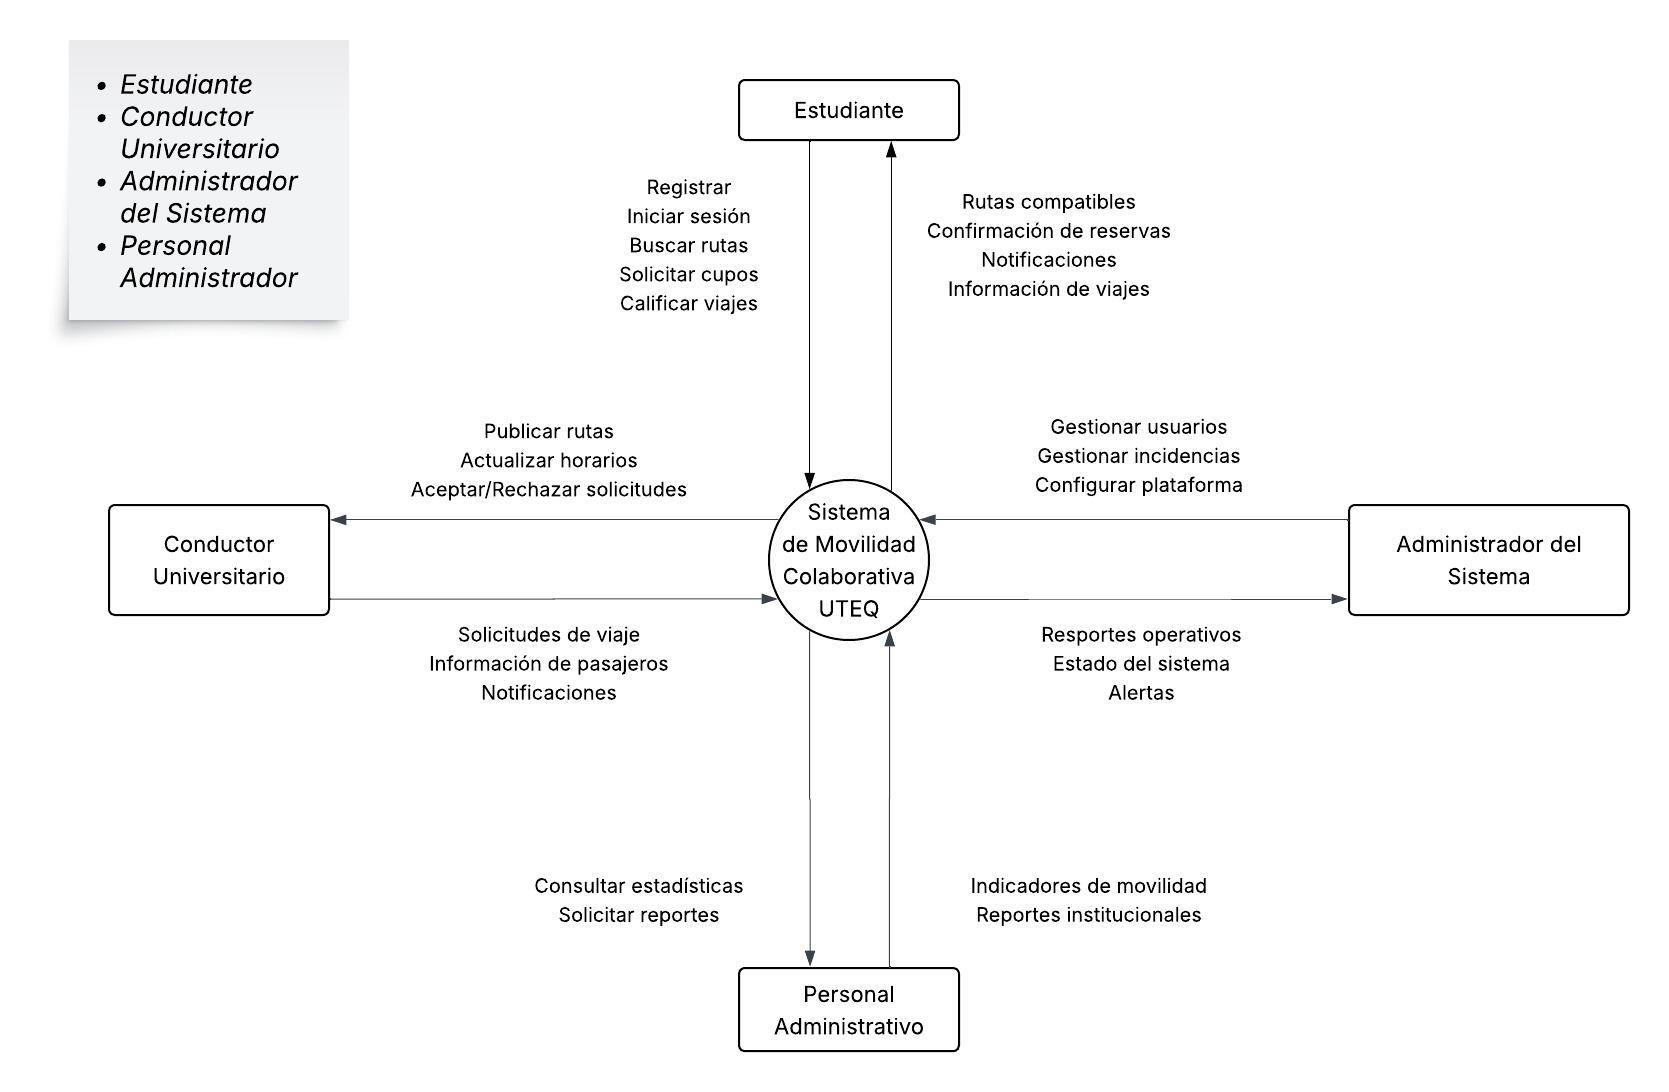
\includegraphics[width=0.99\textwidth]{DIAGRAMA CONTEXTUAL.jpeg}
    \caption{Diagrama de contexto del sistema}
    \label{fig:diagrama_contexto}
\end{figure}

\sline{Funciones del producto}

El Sistema de Movilidad Colaborativa para la Comunidad Universitaria de la UTEQ integra diversas capacidades funcionales diseñadas para optimizar la movilidad estudiantil, fomentar el transporte compartido sostenible y facilitar la coordinación eficiente de viajes entre los campus universitarios. Las funciones principales se enumeran a continuación:

\textbf{Gestión de identidad y acceso:} Administración centralizada de cuentas y niveles de acceso para estudiantes, conductores universitarios, administradores y personal administrativo dentro de la plataforma. El sistema valida las credenciales mediante integración con la API de autenticación de la UTEQ, garantizando que únicamente los miembros activos de la comunidad universitaria puedan acceder a la plataforma. Incluye control de roles y permisos diferenciados según el perfil del usuario, asegurando que cada tipo de usuario tenga acceso únicamente a las operaciones y datos correspondientes a su rol, protegiendo así la confidencialidad de la información.

\textbf{Gestión de perfiles y preferencias:} Registro de datos personales (nombres, apellidos, correo institucional, número de teléfono, fotografía) y preferencias de viaje (rutas frecuentes, horarios preferidos, zonas de recogida) para personalizar la experiencia de movilidad. Los conductores pueden registrar su vehículo documentando marca, modelo, año, color, placa, capacidad de pasajeros y tipo de combustible, permitiendo la publicación de rutas de transporte compartido de manera verificada.

\textbf{Publicación y gestión de rutas: }Los conductores pueden publicar una ruta especificando origen (con geolocalización precisa), destino, fecha, hora de salida, número de cupos disponibles (1-4), y observaciones adicionales. La publicación queda disponible para todos los estudiantes en el motor de búsqueda. Los conductores pueden modificar horarios, cupos o cancelar completamente un viaje, con notificación automática a los pasajeros que hayan realizado reservas afectadas. Las rutas publicadas son visibles en el mapa interactivo y en listados ordenados por proximidad, horario y relevancia.

\textbf{Búsqueda y reserva de viajes:} Los estudiantes pueden buscar viajes disponibles utilizando múltiples filtros: origen (con geolocalización), destino, fecha, hora de salida, precio máximo y calificación mínima del conductor. Los resultados se muestran ordenados por relevancia, cercanía a la ubicación del usuario y compatibilidad con sus preferencias. Los estudiantes pueden reservar un cupo en una ruta publicada, seleccionando la cantidad de cupos deseados según disponibilidad. La reserva se confirma automáticamente si hay cupos disponibles, y el sistema actualiza los cupos restantes en tiempo real, evitando reservas duplicadas. Se implementa un sistema de colas de espera para rutas completas, permitiendo a los estudiantes inscribirse para ser notificados si se libera un cupo.

\textbf{Gestión de viajes activos: }Visualización de la ubicación del conductor durante el trayecto mediante GPS en tiempo real, permitiendo a los pasajeros conocer el estado del viaje y estimar el tiempo de llegada. Tanto conductores como pasajeros pueden cancelar un viaje o una reserva, siempre que se cumplan las políticas de cancelación definidas (ej. cancelación con al menos 2 horas de anticipación). El sistema notifica a todos los involucrados sobre la cancelación, registra la incidencia para el historial y aplica penalizaciones en caso de incumplimiento reiterado. Los pasajeros y conductores pueden coordinar puntos de encuentro específicos para facilitar la recogida y evitar confusiones.

\textbf{Historial y trazabilidad de viajes:} Acceso organizado y cronológico a los antecedentes de viajes realizados, reservas, cancelaciones, calificaciones y observaciones de conductores y pasajeros, permitiendo a los usuarios y administradores revisar el comportamiento y las tendencias de movilidad. Documentación de cada viaje completado con fecha, hora, ruta, conductor, pasajeros, calificación y comentarios, garantizando la trazabilidad de las interacciones. Los usuarios pueden consultar estadísticas personales consolidadas sobre su actividad en la plataforma: número de viajes realizados, tasa de cumplimiento, calificaciones promedio, rutas más frecuentes y horas de mayor actividad.

\textbf{Recomendación inteligente y análisis de datos:} El sistema utiliza algoritmos de inteligencia artificial (aprendizaje automático y filtrado colaborativo) para recomendar a los estudiantes las rutas de transporte compartido que mejor se adapten a sus preferencias y patrones de viaje, considerando factores como historial de viajes, ubicación frecuente, horarios preferidos, calificaciones de conductores, disponibilidad de cupos y condiciones de tráfico. El sistema procesa los datos históricos de viajes para identificar patrones de movilidad recurrentes: rutas más solicitadas, horarios de mayor demanda, días de la semana con mayor actividad y tendencias estacionales. Se realiza detección automática de los horarios y días de la semana con mayor concentración de solicitudes de viaje, permitiendo a los conductores planificar sus publicaciones y a los administradores diseñar estrategias de fomento del carpooling. El sistema también predice la probabilidad de que una ruta en una determinada franja horaria tenga cupos disponibles.

\textbf{Comunicación y notificaciones:} El sistema envía notificaciones push a los dispositivos móviles de los usuarios para informarles sobre confirmación de reserva, cancelación de viaje, recordatorio de viaje próximo (15 minutos antes), alerta de disponibilidad de cupos en rutas frecuentes, y cambios en el estado de una ruta. Los conductores y pasajeros pueden comunicarse a través de un chat interno seguro, sin necesidad de compartir números de teléfono personales, facilitando la coordinación de detalles del viaje y manteniendo un registro de las comunicaciones para resolver disputas. Se distribuyen avisos automáticos con 24 horas, 2 horas y 15 minutos de anticipación al viaje para fomentar la adherencia a las rutas programadas.

\textbf{Calificación y reputación: }Los conductores y pasajeros pueden calificar la experiencia de viaje al finalizar cada trayecto, utilizando una escala de 1 a 5 estrellas y comentarios cualitativos. La calificación promedio se refleja en el perfil del usuario, construyendo un sistema de reputación que fomenta el comportamiento responsable. Los usuarios acumulan puntos de reputación basados en sus calificaciones, cumplimiento de políticas y participación activa en la plataforma. Los usuarios con alta reputación obtienen beneficios como prioridad en la visualización de rutas y acceso a funcionalidades premium. Los administradores pueden revisar calificaciones y comentarios para mediar en conflictos entre conductores y pasajeros.

\textbf{Administración y control:} Los administradores del sistema disponen de un panel completo para gestionar usuarios (activación, desactivación, modificación de roles), rutas (revisión, bloqueo, eliminación), incidencias reportadas y configuración general de la plataforma. Los usuarios pueden reportar incidencias relacionadas con viajes, problemas técnicos o sugerencias de mejora, y el administrador gestiona el flujo de resolución manteniendo un registro de seguimiento. El sistema genera reportes sobre uso de la plataforma (número de viajes, usuarios activos, tasa de reserva, tasa de cancelación), indicadores de movilidad (rutas más usadas, horarios pico, zonas de mayor demanda) y satisfacción de usuarios (calificaciones promedio, comentarios recurrentes). Los datos de movilidad anonimizados pueden ser exportados en formatos estándar (CSV, Excel, PDF) para análisis institucionales. Se mantiene un registro detallado de auditoría de todas las acciones relevantes realizadas por los usuarios y administradores.

\textbf{Seguridad y privacidad:} El sistema cumple con los principios de privacidad y protección de datos, garantizando que la información personal de los usuarios sea almacenada de forma segura mediante encriptación AES-256, accesible solo por usuarios autorizados y utilizada exclusivamente para los fines establecidos en las políticas de privacidad. Los datos utilizados para análisis de movilidad y generación de reportes son anonimizados, eliminando cualquier información que pueda identificar a un usuario individual. Se implementa gestión de permisos específicos para que usuarios autorizados visualicen información de movilidad bajo consentimiento explícito. El sistema solicita consentimiento explícito antes de utilizar funcionalidades que requieran acceso a datos sensibles como ubicación, manteniendo un registro de los consentimientos otorgados.

\textbf{Documentación de observaciones cualitativas:} Los conductores y pasajeros pueden documentar observaciones cualitativas sobre la experiencia de viaje: cumplimiento de horarios, comportamiento del pasajero, condiciones de la ruta y recomendaciones para otros usuarios, enriqueciendo el sistema de reputación y proporcionando información valiosa para la mejora continua de la plataforma. Los administradores pueden registrar notas internas sobre incidentes, decisiones de moderación y observaciones sobre el comportamiento de usuarios específicos.

\textbf{Servicio de notificaciones y recordatorios: }Distribución de avisos automáticos al dispositivo del usuario para fomentar la adherencia a los viajes programados y reducir las cancelaciones de última hora. Los estudiantes pueden suscribirse a alertas para rutas específicas, recibiendo notificaciones cuando un conductor publique un viaje compatible, aumentando las oportunidades de encontrar transporte.

\textbf{Almacenamiento centralizado de datos: }Infraestructura de base de datos centralizada que garantiza la integridad, disponibilidad y seguridad de todos los datos generados por la plataforma: usuarios, rutas, reservas, historial, calificaciones, incidencias y configuraciones. El sistema implementa políticas de backup diario y procedimientos de recuperación ante desastres para garantizar la continuidad del servicio. Se aplican políticas de retención y eliminación de datos que garantizan que la información personal sea conservada únicamente durante el tiempo necesario.

\textbf{Sistema de incentivos y gamificación:} Los usuarios acumulan puntos por participar activamente en la plataforma: publicar rutas, completar viajes, obtener calificaciones positivas y cumplir con las políticas de cancelación. Los puntos pueden canjearse por beneficios como prioridad en la visualización de rutas, acceso a funcionalidades premium y reconocimiento en la comunidad. Se visualizan rankings de conductores y pasajeros más activos y mejor calificados, fomentando una competencia saludable. El sistema ofrece desafíos temáticos que los usuarios pueden completar para desbloquear logros y obtener puntos adicionales.

\sline{Clases y características de usuarios}

\begin{table}[h]
    \centering
    \caption{Perfiles de usuario}
    \label{tab:perfiles}
    \vspace{6pt}
    \begin{tabularx}{\textwidth}{|l|X|X|X|}
    \hline
    \textbf{Usuario} & \textbf{Descripción} & \textbf{Conocimientos} & \textbf{Permisos} \\
    \hline
    Estudiante & Usuario principal que utiliza la plataforma para coordinar traslados & Básico & Publicar solicitudes, buscar rutas, reservar viajes \\
    \hline
    Conductor universitario & Miembro de la comunidad que ofrece transporte compartido & Básico & Publicar rutas, gestionar viajes, coordinar pasajeros \\
    \hline
    Administrador & Responsable de la administración del sistema & Técnico & Gestionar usuarios, monitorear incidencias, configurar parámetros \\
    \hline
    Personal administrativo & Usuario institucional que requiere información & Básico & Consultar estadísticas y reportes \\
    \hline
    \end{tabularx}
\end{table}

\sline{Mapa de stakeholders}

El mapa de stakeholders permite identificar y clasificar a las partes interesadas según su grado de poder e interés, estableciendo estrategias de gestión adecuadas y anticipando posibles conflictos para facilitar su mitigación.

\begin{table}[h]
    \centering
    \caption{Matriz de interés e influencia de los stakeholders}
    \label{tab:stakeholders}
    \vspace{6pt}
    \begin{tabularx}{\textwidth}{|l|c|c|X|}
    \hline
    \textbf{Stakeholder} & \textbf{Interés} & \textbf{Influencia} & \textbf{Estrategia de Gestión} \\
    \hline
    Estudiantes & Alto & Alto & Gestionar de cerca. Realizar pruebas de usabilidad periódicas y encuestas de satisfacción. \\
    \hline
    Administradores del sistema & Alto & Alto & Gestionar de cerca. Proporcionar herramientas de gestión eficaces y capacitación continua. \\
    \hline
    Conductores universitarios & Alto & Medio & Mantener involucrados. Implementar incentivos y mantener comunicación activa. \\
    \hline
    Personal administrativo & Medio & Medio & Mantener informados. Proporcionar reportes claros y actualizados. \\
    \hline
    Docentes & Medio & Bajo & Monitorear. Informar sobre beneficios del sistema y facilitar su uso. \\
    \hline
    Equipo desarrollador & Alto & Medio & Coordinar requisitos, evidencias y trazabilidad del proyecto. \\
    \hline
    \end{tabularx}
\end{table}

\begin{table}[h]
    \centering
    \caption{Matriz Poder-Interés}
    \label{tab:matriz_poder_interes}
    \vspace{6pt}
    \begin{tabularx}{\textwidth}{|l|c|c|X|}
    \hline
    \textbf{Stakeholder} & \textbf{Poder} & \textbf{Interés} & \textbf{Estrategia} \\
    \hline
    Estudiantes & Alto & Alto & Gestionar de cerca. \\
    \hline
    Administradores del sistema & Alto & Alto & Gestionar de cerca. \\
    \hline
    Conductores universitarios & Medio & Alto & Mantener involucrados. \\
    \hline
    Personal administrativo & Medio & Medio & Mantener informados. \\
    \hline
    Docentes & Bajo & Medio & Monitorear. \\
    \hline
    \end{tabularx}
\end{table}
\vspace{6pt}

\newpage
\sline{Entorno operativo}

El Sistema de Movilidad Colaborativa para la Comunidad Universitaria de la UTEQ funcionará en un ecosistema tecnológico distribuido que permite la interacción entre los usuarios (estudiantes, conductores, administradores) y la plataforma a través de dispositivos móviles y computadoras de escritorio.

El entorno operativo se desglosa en los siguientes componentes fundamentales:

\textbf{Plataforma de acceso y dispositivos:} El sistema está diseñado para ejecutarse como una aplicación móvil (Android) y como una plataforma web accesible desde computadoras de escritorio. La aplicación móvil será desarrollada utilizando React Native para garantizar la compatibilidad multiplataforma, permitiendo a los usuarios interactuar con la interfaz de manera fluida desde cualquier dispositivo. Para el acceso web, se requiere un navegador actualizado que permita la visualización de rutas, mapas, reportes y la gestión administrativa de la plataforma.

\textbf{Dispositivo de geolocalización (GPS):} El entorno debe contar con un dispositivo móvil con módulo GPS funcional, el cual es indispensable para la geolocalización en tiempo real de conductores y pasajeros, facilitando la publicación y búsqueda de rutas. El correcto funcionamiento de la geolocalización está supeditado a condiciones mínimas de visibilidad satelital y precisión del receptor GPS.

\textbf{Conectividad:} Se requiere una conexión a Internet estable (Wi-Fi o datos móviles) para permitir la comunicación en tiempo real entre los usuarios, la sincronización de datos con el servidor, el envío de notificaciones push y la integración con los servicios externos de la infraestructura. La conectividad es fundamental para garantizar la experiencia fluida de la plataforma.

\textbf{Infraestructura de servidor y procesamiento:} El sistema se organiza en torno a una unidad central que actúa como servidor web/API, encargada de procesar las peticiones, gestionar la lógica de negocio y coordinar el intercambio de información entre los actores y los módulos externos. El servidor gestiona la autenticación de usuarios, la publicación y búsqueda de rutas, las reservas, el historial de viajes y los reportes administrativos.

\textbf{Módulo de recomendación inteligente (IA):} El procesamiento de datos para la recomendación de rutas y el análisis de patrones de movilidad se delega a un módulo de inteligencia artificial especializado en aprendizaje automático y filtrado colaborativo, el cual devuelve los resultados de las recomendaciones al sistema central. Este módulo procesa datos históricos de viajes para identificar patrones de movilidad, horarios de alta demanda y sugerir rutas compatibles con las preferencias del usuario.

\textbf{Gestión de datos y evidencias:} El entorno operativo incluye una base de datos centralizada para el almacenamiento persistente de la información de usuarios, rutas, reservas, historial de viajes, calificaciones, incidencias y configuraciones. Asimismo, el sistema dispone de un esquema de almacenamiento seguro para conservar las evidencias de cumplimiento y los registros de auditoría de las operaciones realizadas en la plataforma.

\textbf{Servicios externos de soporte:} El sistema interactúa con servicios externos especializados: la API de autenticación de la UTEQ para validar credenciales institucionales, la API de mapas (Google Maps o Mapbox) para renderización de mapas y cálculo de distancias, y un servicio de notificaciones push (Firebase Cloud Messaging) encargado de distribuir avisos, alertas y recordatorios a los dispositivos de los usuarios.

\newpage
\sline{Suposiciones y dependencias}

Esta sección describe los factores externos y las condiciones que se consideran verdaderas para el diseño y éxito del Sistema de Movilidad Colaborativa para la Comunidad Universitaria de la UTEQ, así como los elementos de los cuales depende su operatividad.

\begin{table}[h]
    \centering
    \caption{Suposiciones}
    \label{tab:suposiciones}
    \vspace{6pt}
    \begin{tabularx}{\textwidth}{|l|X|X|}
    \hline
    \textbf{Código} & \textbf{Suposición} & \textbf{Justificación} \\
    \hline
    SUP-01 & Los estudiantes y conductores cuentan con un teléfono celular o computadora con acceso a internet. & La plataforma está diseñada para ser utilizada en entornos digitales; sin acceso a internet, el sistema no puede funcionar correctamente. \\
    \hline
    SUP-02 & Los usuarios poseen habilidades digitales básicas para navegar en la aplicación móvil y web. & La interfaz de usuario está diseñada para ser intuitiva y accesible, asumiendo que los usuarios pueden realizar operaciones básicas como registrarse, buscar rutas y reservar viajes. \\
    \hline
    SUP-03 & Los conductores universitarios están dispuestos a compartir sus viajes y ofrecer transporte a otros miembros de la comunidad. & El éxito del sistema depende de la participación activa de los conductores. Se asume que los incentivos (económicos, sociales, ambientales) son suficientes para motivar su participación. \\
    \hline
    SUP-04 & Los estudiantes están dispuestos a utilizar el transporte compartido como alternativa a otras opciones de movilidad. & La adopción del sistema por parte de los estudiantes es fundamental para generar un volumen significativo de rutas y reservas. \\
    \hline
    SUP-05 & La información ingresada por los usuarios (ubicación, horarios, preferencias de viaje) es veraz y actualizada. & La calidad de las recomendaciones y la coordinación de viajes depende de la precisión de los datos proporcionados por los usuarios. \\
    \hline
    SUP-06 & Los participantes autorizan el uso académico de datos y evidencias cuando corresponda. & El proyecto se desarrolla con fines académicos; se requiere consentimiento informado para el uso de datos y evidencias. \\
    \hline
    \end{tabularx}
\end{table}

\begin{table}[h]
    \centering
    \caption{Dependencias}
    \label{tab:dependencias}
    \vspace{6pt}
    \begin{tabularx}{\textwidth}{|l|X|X|}
    \hline
    \textbf{Código} & \textbf{Dependencia} & \textbf{Justificación} \\
    \hline
    DEP-01 & Conexión a Internet estable. & Permite la sincronización de datos en tiempo real, el acceso a la plataforma, la integración con servicios externos y el envío de notificaciones push. \\
    \hline
    DEP-02 & Sistema de autenticación de la UTEQ disponible y funcional. & La autenticación institucional es esencial para garantizar que solo los miembros de la comunidad universitaria accedan a la plataforma. \\
    \hline
    DEP-03 & API de mapas (Google Maps o Mapbox) disponible y funcional. & La funcionalidad de búsqueda y recomendación de rutas requiere la integración con un servicio de mapas para renderización, cálculo de distancias y geolocalización. \\
    \hline
    DEP-04 & Servicio de notificaciones push (Firebase Cloud Messaging) funcional. & Las notificaciones son esenciales para mantener a los usuarios informados sobre confirmaciones, cancelaciones y recordatorios de viajes. \\
    \hline
    DEP-05 & Base de datos centralizada disponible y funcional. & Almacena usuarios, perfiles, rutas, reservas, historial, calificaciones, incidencias y configuraciones del sistema. \\
    \hline
    DEP-06 & Servidor/API disponible y funcional. & Procesa las peticiones, gestiona la lógica de negocio y coordina el intercambio de información entre los actores y los módulos externos. \\
    \hline
    DEP-07 & Consentimientos informados registrados para uso de datos. & El sistema no debe utilizar datos personales ni de geolocalización sin autorización previa de los usuarios. \\
    \hline
    DEP-08 & Participación activa de la comunidad universitaria (estudiantes, docentes, personal). & El valor del sistema depende de la cantidad de usuarios y de la disponibilidad de rutas de transporte. \\
    \hline
    \end{tabularx}
\end{table}

\vspace{6pt}

\sline{Modelado organizacional i*: dependencia estratégica}

El modelado organizacional i* (dependencia estratégica) permite representar las relaciones entre los actores del sistema y las metas que persiguen, identificando cómo el Sistema de Movilidad Colaborativa contribuye a los objetivos de la comunidad universitaria.

\begin{figure}[h]
    \centering
    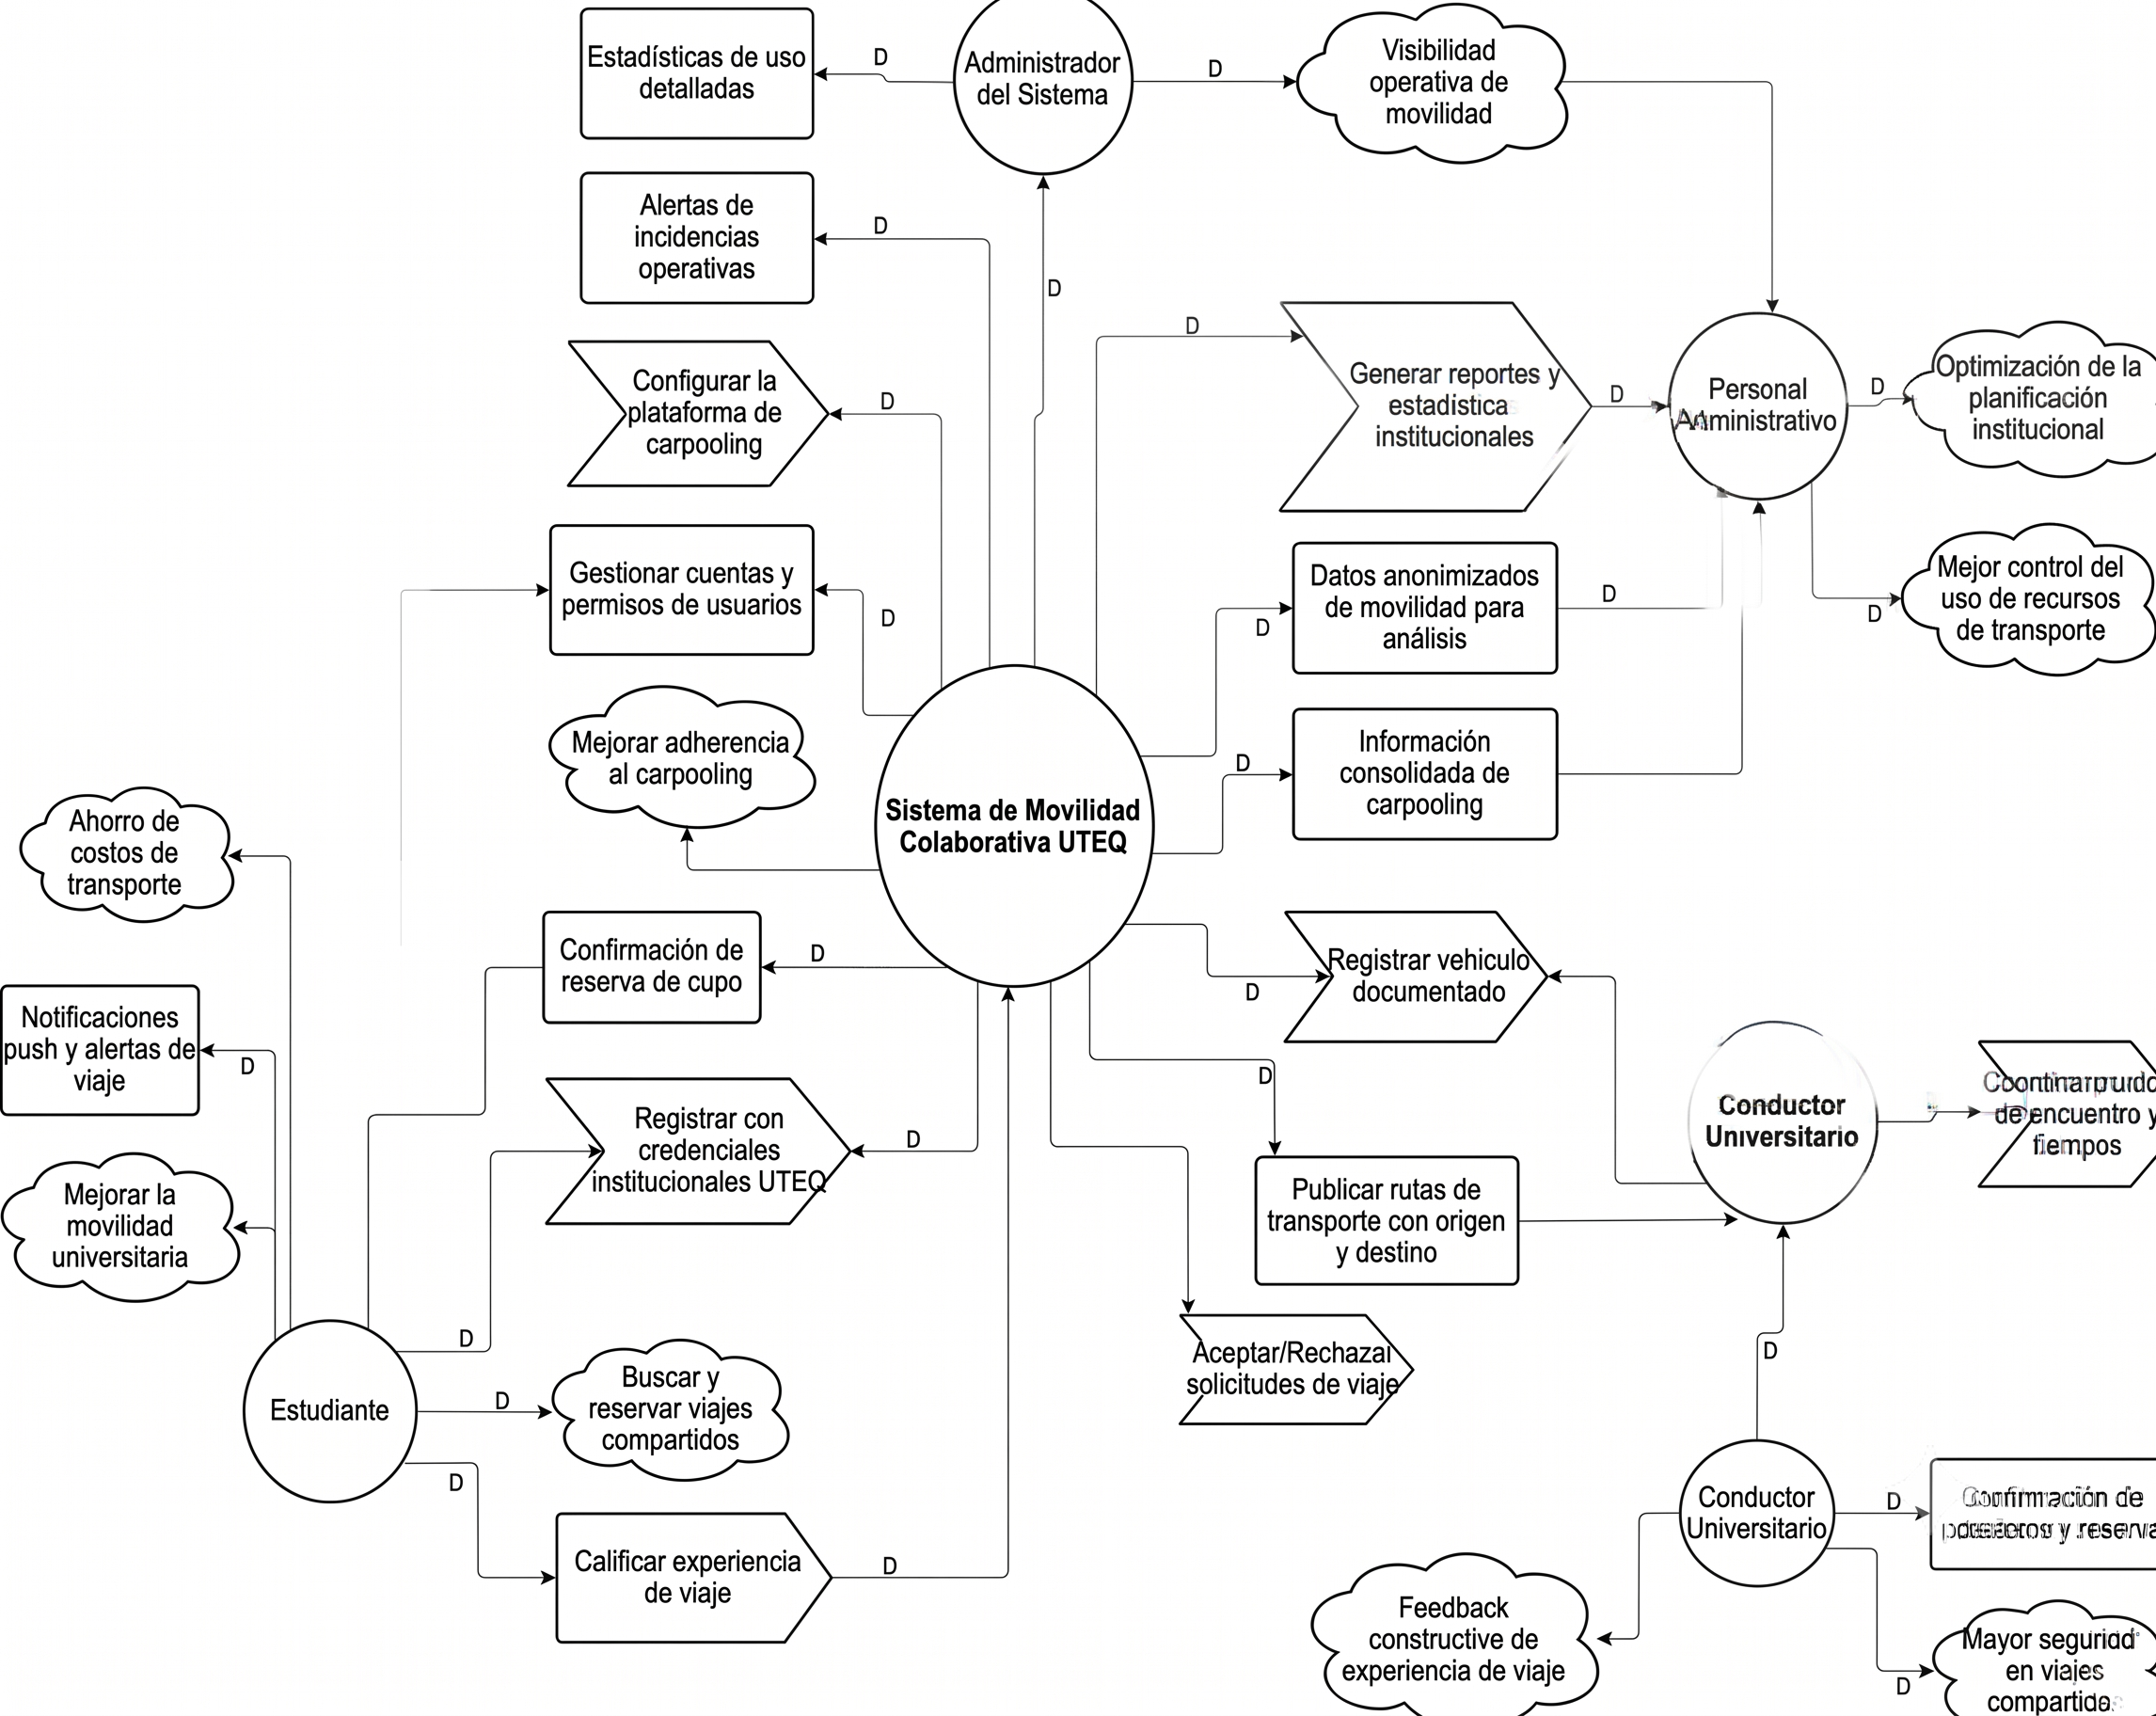
\includegraphics[width=\textwidth]{Diagrama de Dependencia Estratégica.png}
    \caption{Diagrama de Dependencia Estratégica (SD)}
    \label{fig:dependencia_estrategica}
\end{figure}

El diagrama de Dependencia Estratégica representa las relaciones entre estudiantes, conductores universitarios, administradores, personal administrativo y el sistema. Permite identificar metas como mejorar la movilidad estudiantil, optimizar el transporte compartido, reducir costos de desplazamiento, fomentar la sostenibilidad ambiental, gestionar incidencias y generar reportes de movilidad para la toma de decisiones institucionales.

Los actores principales del modelo i* para el Sistema de Movilidad Colaborativa son:

\begin{itemize}
    \item \textbf{Estudiante:} Actor que busca soluciones de transporte económico, seguro y eficiente para trasladarse entre los campus Central y La María. Sus metas principales son acceder a transporte confiable, reducir costos de desplazamiento y optimizar su tiempo de viaje.
    \item \textbf{Conductor universitario:} Actor que ofrece transporte compartido en su vehículo particular. Sus metas principales son compartir costos de combustible y mantenimiento, optimizar el uso de su automóvil y contribuir a una movilidad más sostenible.
    \item \textbf{Administrador del sistema:} Actor responsable de la operación y mantenimiento de la plataforma. Sus metas principales son garantizar el funcionamiento correcto del sistema, gestionar incidencias y asegurar el cumplimiento de las políticas institucionales.
    \item \textbf{Personal administrativo:} Actor institucional que requiere información y reportes de movilidad. Sus metas principales son acceder a estadísticas consolidadas, apoyar la toma de decisiones y planificar políticas de transporte.
    \item \textbf{Sistema de Movilidad Colaborativa:} Actor central que coordina la publicación, búsqueda, reserva y seguimiento de viajes compartidos, facilitando la interacción entre todos los actores.
\end{itemize}

\begin{figure}[h]
    \centering
    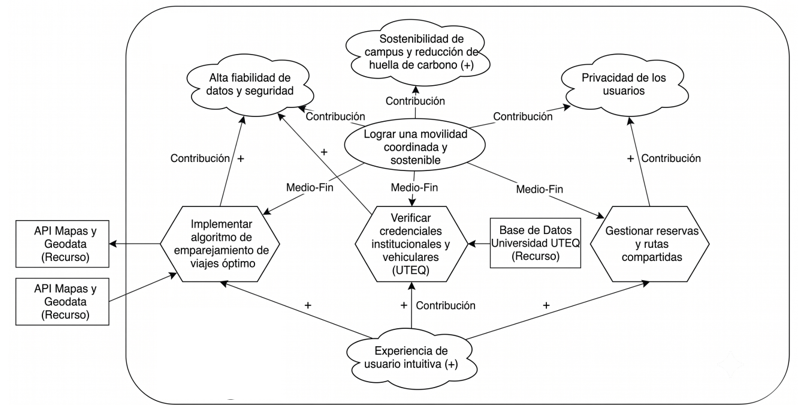
\includegraphics[width=\textwidth]{Diagrama de Justificación Estratégica.png}
    \caption{Diagrama de Justificación Estratégica (SR)}
    \label{fig:justificacion_estrategica}
\end{figure}

El diagrama de Justificación Estratégica muestra cómo el sistema contribuye internamente a las metas del proceso de movilidad colaborativa mediante tareas como autenticar usuarios, publicar rutas, recomendar viajes mediante IA, gestionar reservas, coordinar pasajeros, generar calificaciones y emitir reportes.

Las tareas internas del sistema que contribuyen a las metas estratégicas son:

\begin{itemize}
    \item \textbf{Autenticación institucional:} Valida las credenciales de los usuarios mediante integración con la API de la UTEQ, garantizando que solo miembros de la comunidad universitaria accedan a la plataforma.
    \item \textbf{Publicación de rutas:} Permite a los conductores publicar sus viajes con origen, destino, horario y cupos disponibles, generando la oferta de transporte compartido.
    \item \textbf{Recomendación mediante IA:} Utiliza algoritmos de inteligencia artificial para sugerir a los estudiantes las rutas más compatibles con sus preferencias y patrones de viaje.
    \item \textbf{Gestión de reservas:} Permite a los estudiantes reservar cupos en rutas publicadas, actualizando la disponibilidad en tiempo real y evitando reservas duplicadas.
    \item \textbf{Coordinación de pasajeros:} Facilita la comunicación entre conductores y pasajeros mediante chat interno, permitiendo coordinar puntos de encuentro y detalles del viaje.
    \item \textbf{Calificación y reputación:} Permite a conductores y pasajeros calificar la experiencia de viaje, construyendo un sistema de reputación que fomenta el comportamiento responsable.
    \item \textbf{Generación de reportes:} Produce reportes administrativos sobre uso de la plataforma, indicadores de movilidad y satisfacción de usuarios, apoyando la toma de decisiones institucionales.
    \item \textbf{Gestión de incidencias:} Permite reportar y gestionar incidencias operativas, garantizando la resolución oportuna de problemas y la mejora continua de la plataforma.
\end{itemize}

Las dependencias estratégicas entre actores se establecen de la siguiente manera:

\begin{itemize}
    \item \textbf{Estudiante depende del Sistema:} Para encontrar rutas disponibles, reservar viajes y coordinar su transporte de manera eficiente.
    \item \textbf{Conductor depende del Sistema:} Para publicar sus rutas, gestionar pasajeros y compartir costos de manera organizada.
    \item \textbf{Administrador depende del Sistema:} Para monitorear la operación, gestionar usuarios y generar reportes que faciliten la administración.
    \item \textbf{Personal administrativo depende del Sistema:} Para acceder a información consolidada y estadísticas que apoyen la planificación institucional.
    \item \textbf{Sistema depende de los Actores:} Para generar datos de movilidad que alimenten los algoritmos de recomendación y los reportes administrativos.
\end{itemize}

El modelo i* permite visualizar cómo el Sistema de Movilidad Colaborativa actúa como un facilitador de las metas de los diferentes actores, contribuyendo a la mejora de la movilidad universitaria, la optimización del transporte compartido y la generación de información valiosa para la toma de decisiones institucionales.

\newpage
% =====================================================================
%  3. REQUISITOS ESPECÍFICOS
% =====================================================================

\secband{REQUISITOS ESPECÍFICOS}

La presente sección especifica el comportamiento esperado del sistema a nivel de interacción con usuarios, dispositivos y módulos de software. También formaliza los requisitos funcionales derivados de los requisitos crudos de la 1A, define requisitos no funcionales cuantificados bajo el modelo de calidad ISO/IEC 25010 y establece restricciones de diseño necesarias para proteger la seguridad, privacidad y alcance académico del sistema.

De acuerdo con la estructura ERS/SRS de la Entrega 1B, esta sección cubre: interfaces externas, requisitos funcionales, requisitos no funcionales y restricciones de diseño. Los requisitos se redactan de manera verificable, trazable y con criterios de aceptación comprobables.

% =====================================================================
%  3.1 INTERFACES EXTERNAS
% =====================================================================

\sline{Interfaces externas}

Las interfaces externas describen la forma en que el sistema se comunica con sus usuarios, dispositivos físicos y componentes de software. Esta sección permite identificar qué pantallas se requieren, qué información recibe y entrega el sistema, qué hardware condiciona su funcionamiento y qué módulos de software participan en la solución.

% ---------------------------------------------------------------------
%  3.1.1 Interfaces de usuario
% ---------------------------------------------------------------------

\ssline{Interfaces de usuario}

El sistema contará con interfaces diferenciadas según el rol: estudiante, conductor universitario, administrador y personal administrativo. Cada interfaz deberá mostrar únicamente la información y funciones permitidas para el usuario autenticado. Las pantallas descritas a continuación constituyen la base para la elaboración de mockups y para la trazabilidad con los requisitos funcionales.

\vspace{6pt}
\noindent
\begin{tabular}{|>{\raggedright\arraybackslash}p{2.5cm}|>{\raggedright\arraybackslash}p{2.2cm}|>{\raggedright\arraybackslash}p{3.2cm}|>{\raggedright\arraybackslash}p{3cm}|>{\raggedright\arraybackslash}p{1.8cm}|}
\hline
\rowcolor{uteqgreen!40} \textbf{Pantalla} & \textbf{Usuario principal} & \textbf{Datos de entrada} & \textbf{Datos de salida} & \textbf{RF} \\
\hline
Inicio de sesión & Todos los usuarios & Correo institucional, contraseña y rol & Acceso o mensaje de error & RF-01, RF-02 \\
\hline
Recuperación de contraseña & Todos los usuarios & Correo institucional registrado & Confirmación y enlace de recuperación & RF-01 \\
\hline
Registro de usuario & Todos los usuarios & Nombres, apellidos, correo, teléfono & Usuario registrado y perfil creado & RF-01, RF-06 \\
\hline
Menú principal & Todos los usuarios & Selección de opción & Acceso a la funcionalidad seleccionada & RF-01, RF-02, RF-03, RF-06, RF-13 \\
\hline
Búsqueda de rutas & Estudiante & Origen, destino, fecha y hora & Listado de rutas con opción de reserva & RF-03, RF-04, RF-13 \\
\hline
Recomendaciones IA & Estudiante & Historial de viajes y preferencias & Lista de rutas recomendadas & RF-03, RF-09 \\
\hline
Mis reservas & Estudiante & Filtros por estado (confirmado, pendiente, cancelado) & Lista de reservas con estado & RF-04, RF-05, RF-07 \\
\hline
Historial de viajes & Todos los usuarios & Filtros por período & Listado cronológico de viajes & RF-05, RF-07 \\
\hline
Mi perfil & Todos los usuarios & Datos personales actualizados & Perfil actualizado & RF-06 \\
\hline
Publicación de ruta & Conductor universitario & Origen, destino, fecha, hora, cupos & Ruta publicada y visible & RF-02 \\
\hline
Panel de administración & Administrador & Selección de módulo & Gestión del sistema & RF-09, RF-10, RF-12, RF-15 \\
\hline
Notificaciones & Todos los usuarios & Eventos del sistema & Notificación push & RF-11 \\
\hline
Reporte de incidencias & Usuarios, Administrador & Descripción, categoría y evidencias & Incidencia registrada & RF-12 \\
\hline
Reportes de movilidad & Administrador, Personal administrativo & Período, indicadores y formato & Reporte generado y exportable & RF-09, RF-10, RF-15 \\
\hline
\end{tabular}

\vspace{12pt}

% ---------------------------------------------------------------------
%  3.1.2 Interfaces de hardware
% ---------------------------------------------------------------------

\ssline{Interfaces de hardware}

El sistema interactuará con los componentes de hardware del dispositivo móvil del usuario, requiriendo acceso al módulo GPS para la geolocalización en tiempo real y a la antena de red para la sincronización con el servidor.

\vspace{6pt}
\noindent
\begin{tabular}{|>{\raggedright\arraybackslash}p{3cm}|>{\raggedright\arraybackslash}p{3.5cm}|>{\raggedright\arraybackslash}p{3.5cm}|>{\raggedright\arraybackslash}p{2cm}|}
\hline
\rowcolor{uteqgreen!40} \textbf{Hardware} & \textbf{Uso en el sistema} & \textbf{Restricción} & \textbf{Requisito} \\
\hline
Dispositivo móvil (celular/tablet) & Acceso a la plataforma, geolocalización y notificaciones & Debe tener GPS funcional y conexión a internet & RF-04, RF-11, RNF-09 \\
\hline
Computadora de escritorio & Acceso web para administración y consulta de reportes & Navegador actualizado y conexión estable & RF-10, RF-15, RNF-09 \\
\hline
Servidor de aplicación & Alojar lógica de negocio, API y servicios principales & Disponible durante pruebas y acceso protegido & RNF-02, RNF-07 \\
\hline
Servidor de base de datos & Almacenar usuarios, rutas, reservas, historial y reportes & Integridad, confidencialidad y control por roles & RNF-06, RNF-08 \\
\hline
Conexión de red & Acceso remoto, notificaciones y transferencia de datos & Estabilidad para carga de pantallas y reservas & RNF-02, RNF-07 \\
\hline
\end{tabular}

\vspace{12pt}

% ---------------------------------------------------------------------
%  3.1.3 Interfaces de software
% ---------------------------------------------------------------------
\newpage
\sline{Mockups principales del sistema}

\vspace{6pt}
\noindent
\begin{tabular}{|>{\raggedright\arraybackslash}p{3cm}|>{\raggedright\arraybackslash}p{3.5cm}|>{\raggedright\arraybackslash}p{3.5cm}|>{\raggedright\arraybackslash}p{2.2cm}|}
\hline
\rowcolor{uteqgreen!40} \textbf{Software o módulo} & \textbf{Propósito} & \textbf{Datos intercambiados} & \textbf{Restricción} \\
\hline
Navegador web & Acceso a la plataforma sin instalación local & Formularios, rutas, reportes, alertas y sesiones & Compatible con Chrome, Edge y Firefox actualizados \\
\hline
Backend/API & Reglas de negocio, validaciones y comunicación & Solicitudes de usuarios, credenciales, rutas y reportes & Autenticación, autorización y validaciones \\
\hline
Base de datos & Persistir información de usuarios, rutas, reservas e historial & Usuarios, perfiles, rutas, reservas, calificaciones e incidencias & Acceso restringido por roles y registro de operaciones \\
\hline
Módulo de autenticación & Control de identidad, roles, permisos y sesiones & Credenciales, tokens/sesión, rol y estado del usuario & Cierre de sesión por inactividad y bloqueo de accesos \\
\hline
Módulo de IA (recomendación) & Análisis de patrones de movilidad y recomendación de rutas & Datos históricos de viajes, preferencias, rutas activas & No reemplaza el criterio del usuario; es de apoyo \\
\hline
API de mapas & Renderización de mapas, geolocalización y cálculo de rutas & Coordenadas, distancias, rutas calculadas & Depende de disponibilidad del servicio externo \\
\hline
Servicio de notificaciones & Envío de recordatorios, alertas y avisos & Mensajes, destinatario, fecha, estado y tipo de alerta & No expone datos sensibles sin autorización \\
\hline
Repositorio GitHub & Control de versiones del documento, diagramas y evidencias & Archivos, commits, carpetas y control de cambios & Estructura organizada y commits verificables \\
\hline
\end{tabular}

\vspace{12pt}
Los siguientes mockups representan una propuesta visual inicial de las pantallas principales. No corresponden a una versión final implementada, sino a una guía de interfaz para validar el flujo de interacción con los stakeholders.

Los mockups presentan un diseño limpio, moderno y responsivo, enfocado en una paleta de colores con acentos verdes institucionales, bordes suavizados y una navegación inferior intuitiva que simula una aplicación móvil nativa.

% ---------------------------------------------------------------------
%  Lista de mockups con sus imágenes y descripciones
% ---------------------------------------------------------------------

\begin{figure}[h]
    \centering
    \includegraphics[width=0.99\textwidth]{"INICIAR SESION.png"}
    \caption{Mockup de inicio de sesión}
    \label{fig:mockup_login}
\end{figure}

Permite validar credenciales institucionales y seleccionar el acceso según rol. Presenta un logotipo circular verde con un birrete universitario, seguido del título "Sistema de Movilidad Colaborativa" y la bajada "Comparte transporte con tu comunidad universitaria UTEQ". Incluye campos para Correo institucional y Contraseña, botón principal verde para "Iniciar sesión", botón secundario para "Registrarse" y enlace para recuperar la contraseña. Requisitos relacionados: RF-01, RF-02, RNF-05.

\vspace{12pt}

\begin{figure}[h]
    \centering
    \includegraphics[width=0.99\textwidth]{"CREAR CUENTA.png"}
    \caption{Mockup de registro de usuario}
    \label{fig:mockup_registro}
\end{figure}

Permite registrar nuevos usuarios en la plataforma. Incluye campos para nombres, apellidos, correo institucional, contraseña, confirmación de contraseña y número de teléfono. Requisitos relacionados: RF-01, RF-06.

\vspace{12pt}
\newpage
\begin{figure}[h]
    \centering
    \includegraphics[width=0.99\textwidth]{"MENU USUARIO.png"}
    \caption{Mockup del menú principal del usuario}
    \label{fig:mockup_menu}
\end{figure}

Pantalla de inicio con un saludo personalizado y un icono de notificaciones. Incluye un menú de accesos rápidos en tarjetas con iconos vectoriales a color: Buscar Rutas, Publicar Ruta, Mis Reservas, Historial, IA Rutas, Incidencias, Perfil y Admin. Dispone de barra de navegación inferior persistente. Requisitos relacionados: RF-01, RF-02, RF-03, RF-06, RF-13.

\vspace{12pt}

\begin{figure}[h]
    \centering
    \includegraphics[width=0.99\textwidth]{"BUSCAR RUTAS.png"}
    \caption{Mockup de búsqueda de rutas}
    \label{fig:mockup_buscar_rutas}
\end{figure}

Permite buscar rutas mediante filtros de origen, destino, fecha y hora, con botón verde "Buscar". Los resultados se muestran en tarjetas detalladas con foto del conductor, nombre, calificación, cupos disponibles, horarios, modelo del vehículo y placa, y botón "Reservar". Requisitos relacionados: RF-03, RF-04, RF-13.
\newpage
\vspace{12pt}

\begin{figure}[h]
    \centering
    \includegraphics[width=0.99\textwidth]{"RECOMENDACIONES IA.png"}
    \caption{Mockup de recomendaciones IA}
    \label{fig:mockup_recomendaciones_ia}
\end{figure}

Pantalla de asistente inteligente con banner "Rutas recomendadas para ti basadas en tus patrones de viaje". Muestra tarjetas de coincidencia con porcentaje de afinidad, duración estimada, calificación del conductor y botón verde "Reservar". Requisitos relacionados: RF-03, RF-09.

\vspace{12pt}

\begin{figure}[h]
    \centering
    \includegraphics[width=0.99\textwidth]{"MIS RESERVAS.png"}
    \caption{Mockup de mis reservas}
    \label{fig:mockup_reservas}
\end{figure}

Lista cronológica de tarjetas con etiquetas de estado en colores pastel: Confirmado (Verde), Pendiente (Naranja), Cancelado (Rojo). Cada tarjeta incluye conductor, ruta, y botones para "Ver detalles" y "Cancelar" según estado. Requisitos relacionados: RF-04, RF-05, RF-07.

\vspace{12pt}
\newpage
\begin{figure}[h]
    \centering
    \includegraphics[width=0.99\textwidth]{"HISTORIAL DE VIAJES.png"}
    \caption{Mockup de historial de viajes}
    \label{fig:mockup_historial}
\end{figure}

Permite consultar el historial completo de viajes realizados, reservados y cancelados, organizado cronológicamente con detalles de cada trayecto. Requisitos relacionados: RF-05, RF-07.

\vspace{12pt}

\begin{figure}[h]
    \centering
    \includegraphics[width=0.99\textwidth]{"MI PERFIL.png"}
    \caption{Mockup de mi perfil}
    \label{fig:mockup_perfil}
\end{figure}

Tarjeta centralizada con foto de perfil, nombre y datos clave con iconos descriptivos: carrera, nivel, correo institucional y teléfono. Incluye botones: "Editar Perfil" (verde), "Cambiar Contraseña" (borde verde) y "Cerrar Sesión" (fondo rosado con texto rojo). Requisitos relacionados: RF-06.

\vspace{12pt}
\newpage
\begin{figure}[h]
    \centering
    \includegraphics[width=0.99\textwidth]{"PANEL DE ADMINISTRACION.png"}
    \caption{Mockup del panel de administración}
    \label{fig:mockup_panel_admin}
\end{figure}

Panel con menú lateral izquierdo (Dashboard, Usuarios, Rutas, Incidencias, Reportes, Configuración). Incluye métricas principales (Usuarios 1,245, Conductores 89, Rutas 156, Reservas 432, Incidencias 12, Reportes 28), gráficos de barras para Viajes por día y gráfico de dona para Tipo de transporte, y tabla de Incidencias recientes. Requisitos relacionados: RF-09, RF-10, RF-12, RF-15.

\vspace{12pt}

\begin{figure}[h]
    \centering
    \includegraphics[width=0.99\textwidth]{"NOTIFICACIONES.png"}
    \caption{Mockup de notificaciones}
    \label{fig:mockup_notificaciones}
\end{figure}

Historial de alertas en tarjetas con viñetas de color: Verde (confirmación de reserva), Amarillo (actualización de horarios), Rojo (viajes cancelados). Incluyen marcas de tiempo relativas ("Hace 5 min", "Hace 1 hora"). Requisitos relacionados: RF-11.

\vspace{12pt}
\newpage
\begin{figure}[h]
    \centering
    \includegraphics[width=0.99\textwidth]{"REPORTAR INCIDENCIAS.png"}
    \caption{Mockup de reporte de incidencias}
    \label{fig:mockup_incidencias}
\end{figure}

Formulario con banner naranja de advertencia, menú desplegable para Tipo de incidencia, caja de texto para Descripción, selector para adjuntar evidencias, campo de fecha y geolocalización. Botón naranja "Enviar Reporte". Requisitos relacionados: RF-12.
\newpage
% =====================================================================
%  3.3 COBERTURA DE MOCKUPS FRENTE A INTERFACES Y REQUISITOS
% =====================================================================

\sline{Cobertura de mockups frente a interfaces y requisitos}

La siguiente tabla verifica que cada mockup incluido en la sección 3.1 representa una interfaz concreta, tiene un usuario principal definido y se relaciona con requisitos funcionales del sistema. Esta matriz evita que los mockups queden como imágenes aisladas y facilita la trazabilidad interna de la sección.
\begin{center}
\small
\begin{tabular}{|>{\raggedright\arraybackslash}p{2.3cm}|>{\raggedright\arraybackslash}p{3.5cm}|>{\raggedright\arraybackslash}p{2.8cm}|>{\raggedright\arraybackslash}p{3.2cm}|>{\raggedright\arraybackslash}p{1.8cm}|}
\hline
\textbf{Mockup} & \textbf{Interfaz representada} & \textbf{Usuario principal} & \textbf{RF cubiertos} & \textbf{Estado} \\
\hline
\scriptsize INICIAR SESION & Inicio de sesión & Todos los usuarios & RF-01, RF-02 & Cubierto \\
\hline
\scriptsize CREAR CUENTA & Registro de usuario & Todos los usuarios & RF-01, RF-06 & Cubierto \\
\hline
\scriptsize MENU USUARIO & Menú principal / Dashboard & Todos los usuarios & RF-01, RF-02, RF-03, RF-06, RF-13 & Cubierto \\
\hline
\scriptsize BUSCAR RUTAS & Búsqueda de rutas & Estudiante & RF-03, RF-04, RF-13 & Cubierto \\
\hline
\scriptsize RECOMENDACIONES IA & Recomendaciones IA & Estudiante & RF-03, RF-09 & Cubierto \\
\hline
\scriptsize MIS RESERVAS & Mis reservas & Estudiante & RF-04, RF-05, RF-07 & Cubierto \\
\hline
\scriptsize HISTORIAL DE VIAJES & Historial de viajes & Todos los usuarios & RF-05, RF-07 & Cubierto \\
\hline
\scriptsize MI PERFIL & Mi perfil & Todos los usuarios & RF-06 & Cubierto \\
\hline
\scriptsize PANEL DE ADMINISTRACION & Panel de administración & Administrador & RF-09, RF-10, RF-12, RF-15 & Cubierto \\
\hline
\scriptsize NOTIFICACIONES & Notificaciones & Todos los usuarios & RF-11 & Cubierto \\
\hline
\scriptsize REPORTAR INCIDENCIAS & Reporte de incidencias & Usuarios, Administrador & RF-12 & Cubierto \\
\hline
\end{tabular}
\end{center}

Los mockups presentados cubren las interfaces principales del sistema para los diferentes roles: estudiantes (búsqueda, reserva, recomendaciones IA, historial, perfil), conductores (publicación de rutas, gestión de reservas), administradores (panel de control, gestión de usuarios, reportes) y todos los usuarios (inicio de sesión, registro, notificaciones). Cada mockup ha sido diseñado considerando los requisitos funcionales correspondientes y las necesidades específicas de cada perfil de usuario, manteniendo una experiencia de usuario consistente y alineada con la identidad visual institucional de la UTEQ.
\newpage
% =====================================================================
%  4. MODELADO DEL SISTEMA (UML)
% =====================================================================

\secband{MODELADO DEL SISTEMA (UML)}

\sline{Diagrama de casos de uso general}

\begin{figure}[h]
    \centering
    \includegraphics[width=\textwidth]{diagrama_casos_uso.png}
    \caption{Diagrama de casos de uso general}
    \label{fig:casos_uso}
\end{figure}

\sline{Especificación textual de casos de uso}

\textbf{Caso de Uso 1: Autenticación de usuarios}

\begin{tabularx}{\textwidth}{|l|X|}
\hline
\textbf{Campo} & \textbf{Descripción} \\
\hline
ID & CU-01 \\
\hline
Nombre & Autenticación de usuarios institucionales \\
\hline
Actor & Estudiante, Conductor Universitario \\
\hline
Descripción & El usuario ingresa sus credenciales institucionales para acceder al sistema \\
\hline
Precondición & El usuario debe tener un correo institucional activo \\
\hline
Postcondición & El usuario accede al sistema con permisos según su rol \\
\hline
Flujo básico & 1. El usuario ingresa correo y contraseña \newline 2. El sistema valida con la API UTEQ \newline 3. La UTEQ confirma la autenticación \newline 4. El sistema redirige al dashboard correspondiente \\
\hline
Flujos alternativos & 1a. Si las credenciales son incorrectas, se muestra mensaje de error \newline 1b. Si la cuenta está inactiva, se bloquea el acceso \\
\hline
\end{tabularx}

\textbf{Caso de Uso 2: Publicación de ruta}

\begin{tabularx}{\textwidth}{|l|X|}
\hline
\textbf{Campo} & \textbf{Descripción} \\
\hline
ID & CU-02 \\
\hline
Nombre & Publicación de ruta de transporte \\
\hline
Actor & Conductor Universitario \\
\hline
Descripción & El conductor publica una ruta con origen, destino, horario y cupos \\
\hline
Precondición & El conductor debe tener su vehículo registrado \\
\hline
Postcondición & La ruta queda visible para los estudiantes \\
\hline
Flujo básico & 1. El conductor selecciona publicar viaje \newline 2. Ingresa origen, destino, hora y asientos \newline 3. Confirma la publicación \newline 4. El sistema almacena la ruta y notifica a los interesados \\
\hline
Flujos alternativos & 2a. Si falta algún dato obligatorio, no permite publicar \\
\hline
\end{tabularx}

\textbf{Caso de Uso 3: Reserva de viaje}

\begin{tabularx}{\textwidth}{|l|X|}
\hline
\textbf{Campo} & \textbf{Descripción} \\
\hline
ID & CU-03 \\
\hline
Nombre & Reserva de viaje compartido \\
\hline
Actor & Estudiante \\
\hline
Descripción & El estudiante reserva un cupo en una ruta publicada \\
\hline
Precondición & La ruta debe tener cupos disponibles \\
\hline
Postcondición & El cupo queda reservado y el conductor es notificado \\
\hline
Flujo básico & 1. El estudiante selecciona una ruta \newline 2. Confirma la reserva \newline 3. El sistema actualiza cupos \newline 4. Se envía notificación al conductor \\
\hline
Flujos alternativos & 2a. Si no hay cupos, se muestra mensaje de ruta completa \\
\hline
\end{tabularx}

\textbf{Caso de Uso 4: Cancelación de viaje}

\begin{tabularx}{\textwidth}{|l|X|}
\hline
\textbf{Campo} & \textbf{Descripción} \\
\hline
ID & CU-04 \\
\hline
Nombre & Cancelación de viaje \\
\hline
Actor & Conductor, Estudiante \\
\hline
Descripción & El usuario cancela un viaje o una reserva activa \\
\hline
Precondición & El viaje o reserva debe estar activo \\
\hline
Postcondición & El viaje o reserva queda cancelado \\
\hline
Flujo básico & 1. El usuario selecciona cancelar \newline 2. Confirma la cancelación \newline 3. El sistema actualiza el estado \newline 4. Se notifica a los involucrados \\
\hline
Flujos alternativos & 1a. Si la cancelación es cerca de la hora, se requiere confirmación extra \\
\hline
\end{tabularx}

\textbf{Caso de Uso 5: Visualización de historial}

\begin{tabularx}{\textwidth}{|l|X|}
\hline
\textbf{Campo} & \textbf{Descripción} \\
\hline
ID & CU-05 \\
\hline
Nombre & Visualización de historial de viajes \\
\hline
Actor & Todos los usuarios \\
\hline
Descripción & El usuario consulta su historial de viajes realizados y reservados \\
\hline
Precondición & El usuario debe haber iniciado sesión \\
\hline
Postcondición & Se muestra el historial organizado por fecha \\
\hline
Flujo básico & 1. El usuario accede a su historial \newline 2. El sistema consulta los registros \newline 3. Se muestran los viajes organizados \\
\hline
Flujos alternativos & 2a. Si no hay viajes, se muestra mensaje informativo \\
\hline
\end{tabularx}

\sline{Diagrama de clases conceptual}

\begin{figure}[h]
    \centering
    \includegraphics[width=\textwidth]{diagrama_clases.png}
    \caption{Diagrama de clases conceptual}
    \label{fig:diagrama_clases}
\end{figure}

\newpage

% =====================================================================
%  5. PRIORIZACIÓN Y TRAZABILIDAD
% =====================================================================

\secband{PRIORIZACIÓN Y TRAZABILIDAD}

\sline{Clasificación de requisitos}

\begin{table}[h]
    \centering
    \caption{Clasificación de requisitos funcionales}
    \label{tab:clasificacion_rf}
    \vspace{6pt}
    \begin{tabularx}{\textwidth}{|l|X|X|X|}
    \hline
    \textbf{ID} & \textbf{Nombre del requisito} & \textbf{Tipo} & \textbf{Categoría} \\
    \hline
    RF-01 & Autenticación de usuarios institucionales & RF & Seguridad / Acceso \\
    \hline
    RF-02 & Publicación de rutas de transporte & RF & Transporte \\
    \hline
    RF-03 & Recomendación de rutas mediante IA & RF & Inteligencia Artificial \\
    \hline
    RF-04 & Reserva de viaje compartido & RF & Transporte \\
    \hline
    RF-05 & Cancelación de viaje & RF & Transporte \\
    \hline
    RF-06 & Gestión de perfil de usuario & RF & Gestión de usuarios \\
    \hline
    RF-07 & Historial de viajes & RF & Gestión de datos \\
    \hline
    RF-08 & Calificación de viajes & RF & Gestión de usuarios \\
    \hline
    RF-09 & Análisis de patrones de movilidad & RF & Análisis de datos \\
    \hline
    RF-10 & Generación de reportes administrativos & RF & Reportes \\
    \hline
    RF-11 & Notificaciones en tiempo real & RF & Comunicación \\
    \hline
    RF-12 & Gestión de incidencias & RF & Administración \\
    \hline
    RF-13 & Búsqueda avanzada de rutas & RF & Transporte \\
    \hline
    RF-14 & Registro de vehículo & RF & Gestión de usuarios \\
    \hline
    RF-15 & Exportación de datos de movilidad & RF & Reportes \\
    \hline
    \end{tabularx}
\end{table}

\begin{table}[h]
    \centering
    \caption{Clasificación de requisitos no funcionales}
    \vspace{6pt}
    \begin{tabularx}{\textwidth}{|l|X|X|X|}
    \hline
    \textbf{ID} & \textbf{Nombre del requisito} & \textbf{Tipo} & \textbf{Categoría} \\
    \hline
    RNF-01 & Usabilidad / Tiempo de registro & RNF & Calidad ISO/IEC 25010 \\
    \hline
    RNF-02 & Tiempo de carga máximo & RNF & Eficiencia de desempeño \\
    \hline
    RNF-03 & Tiempo de respuesta IA & RNF & Eficiencia / IA \\
    \hline
    RNF-04 & Disponibilidad & RNF & Fiabilidad \\
    \hline
    RNF-05 & Seguridad de datos & RNF & Seguridad \\
    \hline
    RNF-06 & Confidencialidad por roles & RNF & Seguridad / Confidencialidad \\
    \hline
    RNF-07 & Disponibilidad en pruebas & RNF & Fiabilidad / Disponibilidad \\
    \hline
    RNF-08 & Integridad de datos & RNF & Integridad \\
    \hline
    RNF-09 & Compatibilidad & RNF & Compatibilidad \\
    \hline
    RNF-10 & Mantenibilidad & RNF & Mantenibilidad \\
    \hline
    RNF-11 & Accesibilidad & RNF & Accesibilidad / Usabilidad \\
    \hline
    RNF-12 & Privacidad & RNF & Privacidad / Consentimiento \\
    \hline
    \end{tabularx}
\end{table}

\sline{Priorización MoSCoW}

\begin{table}[h]
    \centering
    \caption{Priorización MoSCoW justificada}
    \label{tab:moscow}
    \vspace{6pt}
    \begin{tabularx}{\textwidth}{|l|X|X|X|}
    \hline
    \textbf{ID} & \textbf{Requisito} & \textbf{Prioridad} & \textbf{Justificación} \\
    \hline
    RF-01 & Autenticación de usuarios & Must & Sin autenticación, el sistema no puede operar; es el punto de entrada obligatorio \\
    \hline
    RF-02 & Publicación de rutas & Must & Es la función principal del sistema; sin ella no hay viajes que coordinar \\
    \hline
    RF-04 & Reserva de viaje & Must & Permite a los estudiantes coordinar su transporte; es esencial \\
    \hline
    RF-06 & Gestión de perfil & Must & Los usuarios necesitan gestionar su información personal \\
    \hline
    RF-14 & Registro de vehículo & Must & Los conductores necesitan registrar su vehículo para publicar rutas \\
    \hline
    RF-03 & Recomendación de rutas IA & Should & Mejora la experiencia pero no es indispensable para el funcionamiento básico \\
    \hline
    RF-07 & Historial de viajes & Should & Permite consultar viajes pasados pero no es crítico \\
    \hline
    RF-11 & Notificaciones en tiempo real & Should & Mejora la comunicación pero no es esencial para la operación \\
    \hline
    RF-13 & Búsqueda avanzada & Should & Facilita la búsqueda pero no es indispensable \\
    \hline
    RF-08 & Calificación de viajes & Could & Agrega valor al sistema pero no es crítico \\
    \hline
    RF-10 & Reportes administrativos & Could & Útil para administración pero no esencial para el núcleo \\
    \hline
    RF-15 & Exportación de datos & Could & Funcionalidad adicional para análisis institucional \\
    \hline
    RF-09 & Análisis de patrones & Could & Mejora la planificación pero no es indispensable \\
    \hline
    RF-12 & Gestión de incidencias & Could & Permite gestionar problemas pero no es crítico \\
    \hline
    RF-05 & Cancelación de viaje & Should & Permite flexibilidad pero no es indispensable \\
    \hline
    \end{tabularx}
\end{table}

\sline{Matriz de trazabilidad parcial}

\begin{table}[h]
    \centering
    \caption{Matriz de trazabilidad parcial}
    \label{tab:trazabilidad}
    \vspace{6pt}
    \begin{tabularx}{\textwidth}{|l|l|l|X|}
    \hline
    \textbf{Evidencia (ID-EV)} & \textbf{Requisito (ID)} & \textbf{Caso de Uso (ID)} & \textbf{Descripción} \\
    \hline
    EV-ENT-01 & RF-01, RF-02, RF-04 & CU-01, CU-02, CU-03 & Entrevista a estudiantes sobre necesidades de transporte compartido \\
    \hline
    EV-ENT-02 & RF-03, RF-09, RF-10 & CU-01 & Entrevista a conductores sobre rutas y preferencias \\
    \hline
    EV-ENT-03 & RF-06, RF-07, RF-11 & CU-05 & Entrevista sobre experiencia de usuario y notificaciones \\
    \hline
    EV-CUE-01 & RF-01, RF-02, RF-04 & CU-01, CU-02, CU-03 & Cuestionario sobre movilidad universitaria \\
    \hline
    EV-OBS-01 & RF-09, RF-10 & CU-05 & Observación de patrones de movilidad en la UTEQ \\
    \hline
    EV-CONS-01 & RNF-06, RNF-12 & CU-01 & Consentimiento informado para uso de datos \\
    \hline
    \end{tabularx}
\end{table}

\newpage

% =====================================================================
%  6. CONCLUSIONES
% =====================================================================

\secband{CONCLUSIONES}

\sline{Logros de la entrega}

La Entrega 1B permitió consolidar la primera versión formal del documento ERS/SRS del \textbf{Sistema de Movilidad Colaborativa para la Comunidad Universitaria de la UTEQ}. Se logró transformar las necesidades iniciales de los stakeholders en requisitos funcionales, requisitos no funcionales, restricciones de diseño, modelos UML y mecanismos de trazabilidad.

Se documentaron 15 requisitos funcionales con atributos verificables, 12 requisitos no funcionales cuantificados bajo el enfoque ISO/IEC 25010, y restricciones técnicas, éticas y operativas. También se completó el modelado UML incluyendo diagrama de contexto, casos de uso, clases conceptuales, arquitectura lógica y despliegue.

\sline{Decisiones de diseño tempranas}

Las decisiones de diseño se orientaron a mantener al estudiante como actor central del sistema. El sistema se define como una herramienta de apoyo a la movilidad universitaria, pero no reemplaza la planificación de transporte institucional ni atiende emergencias. Se estableció que el uso de datos personales y geolocalización debe depender de autorización previa y control de roles.

\sline{Trabajo pendiente para la 2A}

Como trabajo pendiente para la Entrega 2A, se considera necesario ampliar el nivel de detalle técnico del diseño, validar los modelos con los stakeholders, refinar los prototipos de interfaz, definir con mayor precisión la arquitectura tecnológica y preparar una versión más cercana a la implementación del sistema.

\newpage

% =====================================================================
%  REFERENCIAS
% =====================================================================

\secband{REFERENCIAS}

[1] S. AlQuhtani, ``Ridesharing as a Potential Sustainable Transportation Alternative in Suburban Universities: The Case of Najran University, Saudi Arabia,'' \textit{Sustainability}, vol. 14, no. 8, p. 4392, 2022.

[2] R. López-Chila, M. Dávila-Moreno, G. Muñoz-Franco, and M. Estrella-Guayasamin, ``Methodology and Innovation in the Design of Shared Transportation Systems for Academic Environments,'' \textit{Sustainability}, vol. 17, 2025.

[3] ISO/IEC, \textit{ISO/IEC/IEEE 29148:2018: Systems and software engineering -- Life cycle processes -- Requirements engineering}. ISO, 2018.

[4] Pressman, R. S. \textit{Software Engineering: A Practitioner's Approach}. 8th ed. McGraw-Hill, 2014.

[5] Sommerville, I. \textit{Software Engineering}. 10th ed. Pearson, 2016.

[6] Wiegers, K. E. and Beatty, J. \textit{Software Requirements}. 3rd ed. Microsoft Press, 2013.

\newpage

% =====================================================================
%  APÉNDICES
% =====================================================================

\secband{APÉNDICES}

\sline{Apéndice A — Plan del proyecto de IR}

\textbf{Cronograma:}

\begin{table}[h]
    \centering
    \caption{Cronograma del proyecto de Ingeniería de Requisitos}
    \vspace{6pt}
    \begin{tabularx}{\textwidth}{|l|X|X|X|}
    \hline
    \textbf{Actividad} & \textbf{Responsable principal} & \textbf{Fecha planificada} & \textbf{Estado} \\
    \hline
    Selección del sistema objetivo & Equipo CMVZ & 28/05/2026 & Completado \\
    \hline
    Identificación de stakeholders & Kevin Contreras & 29/05/2026 & Completado \\
    \hline
    Elaboración de guía de entrevista & Equipo CMVZ & 29/05/2026 & Completado \\
    \hline
    Aplicación de entrevistas & Equipo CMVZ & 30/05/2026 & Completado \\
    \hline
    Análisis de requisitos crudos & Equipo CMVZ & 30/05/2026 & Completado \\
    \hline
    Corrección de observaciones 1A & Equipo CMVZ & 26/06/2026 & Completado \\
    \hline
    Elaboración de requisitos específicos & Angelo Zambrano & 27/06/2026 & Completado \\
    \hline
    Modelado UML funcional & Frixon Morán & 28/06/2026 & Completado \\
    \hline
    Modelado estructural y trazabilidad & Jonathan Viteri & 28/06/2026 & Completado \\
    \hline
    Integración y revisión final & Equipo CMVZ & 29/06/2026 & Completado \\
    \hline
    \end{tabularx}
\end{table}

\textbf{Roles del equipo:}

\begin{table}[h]
    \centering
    \caption{Roles del equipo CMVZ}
    \vspace{6pt}
    \begin{tabularx}{\textwidth}{|l|X|X|}
    \hline
    \textbf{Integrante} & \textbf{Rol asignado} & \textbf{Responsabilidades principales} \\
    \hline
    Cordova Carreño Mayra Lucila & Diseñadora de Modelos & Diagramas UML, mockups y modelado visual \\
    \hline
    Herrera Moran Gilmar Javier & Analista de Requerimientos & Elicitación, análisis de requisitos y documentación \\
    \hline
    Naranjo Flores Anderson Jeampiere & Analista Líder / Gestión de Proyecto & Coordinación, integración y gestión del proyecto \\
    \hline
    Valarezo Flores Steven Alexander & Analista de Requerimientos / Investigador de Campo & Trabajo de campo, entrevistas y evidencias \\
    \hline
    \end{tabularx}
\end{table}

\textbf{Técnicas de elicitación seleccionadas:}

\begin{itemize}
    \item \textbf{Entrevista semiestructurada:} Permitió obtener información detallada sobre necesidades de movilidad, rutas frecuentes y preferencias de transporte.
    \item \textbf{Cuestionario:} Permitió estandarizar preguntas y organizar la información recolectada en categorías temáticas.
    \item \textbf{Observación:} Permitió identificar limitaciones del transporte actual y patrones de movilidad.
    \item \textbf{Revisión documental:} Permitió sustentar el problema con literatura sobre movilidad universitaria y carpooling.
\end{itemize}

\sline{Apéndice B — Trabajo de campo y evidencias}

\ssline{B.1 Registro de evidencias}

\begin{table}[h]
    \centering
    \caption{Catálogo de evidencias del proyecto}
    \vspace{6pt}
    \begin{tabularx}{\textwidth}{|l|X|X|X|}
    \hline
    \textbf{ID de evidencia} & \textbf{Tipo de evidencia} & \textbf{Descripción} & \textbf{Requisitos derivados} \\
    \hline
    EV-ENT-01 & Entrevista & Entrevista a estudiantes sobre necesidades de transporte & RF-01, RF-02, RF-04, RF-07 \\
    \hline
    EV-ENT-02 & Entrevista & Entrevista a conductores sobre rutas y preferencias & RF-03, RF-09, RF-10, RF-14 \\
    \hline
    EV-ENT-03 & Entrevista & Entrevista sobre experiencia de usuario y notificaciones & RF-06, RF-07, RF-11, RF-13 \\
    \hline
    EV-CUE-01 & Cuestionario & Cuestionario sobre movilidad universitaria & RF-01, RF-02, RF-04 \\
    \hline
    EV-OBS-01 & Observación & Observación de patrones de movilidad en la UTEQ & RF-09, RF-10 \\
    \hline
    EV-CONS-01 & Consentimiento & Consentimiento informado firmado por participantes & RNF-06, RNF-12 \\
    \hline
    EV-MUL-01 & Multimedia & Fotos, capturas y evidencias del levantamiento & Apoya trazabilidad general \\
    \hline
    \end{tabularx}
\end{table}

\ssline{B.2 Guía de entrevista}

\textbf{Cuestionario de entrevista - Movilidad Universitaria}

\textbf{1. Necesidades de transporte}
\begin{itemize}
    \item ¿Qué dificultades enfrenta actualmente para trasladarse a la UTEQ?
    \item ¿Con qué frecuencia utiliza transporte para llegar a la universidad?
    \item ¿Considera que el transporte compartido es una alternativa viable?
\end{itemize}

\textbf{2. Rutas y preferencias}
\begin{itemize}
    \item ¿Qué rutas utiliza con mayor frecuencia?
    \item ¿En qué horarios suele trasladarse?
    \item ¿Qué factores considera importantes al elegir un medio de transporte?
\end{itemize}

\textbf{3. Experiencia y tecnología}
\begin{itemize}
    \item ¿Ha utilizado aplicaciones de transporte compartido anteriormente?
    \item ¿Qué funcionalidades considera esenciales en una aplicación de movilidad?
    \item ¿Estaría dispuesto a compartir su ubicación para coordinar viajes?
\end{itemize}

\ssline{B.3 Actas de entrevista firmadas (≥2)}

\begin{table}[h]
    \centering
    \caption{Registro de actas de entrevista}
    \vspace{6pt}
    \begin{tabularx}{\textwidth}{|l|X|X|X|X|}
    \hline
    \textbf{ID de acta} & \textbf{Fecha} & \textbf{Entrevistador} & \textbf{Entrevistado} & \textbf{Evidencias incluidas} \\
    \hline
    ACT-ENT-01 & 30/05/2026 & Valarezo Flores Steven A. & Estudiante UTEQ & Pregunta-respuesta, captura, consentimiento \\
    \hline
    ACT-ENT-02 & 30/05/2026 & Herrera Moran Gilmar J. & Conductor universitario & Pregunta-respuesta, captura, consentimiento \\
    \hline
    ACT-ENT-03 & 30/05/2026 & Naranjo Flores Anderson J. & Personal administrativo & Pregunta-respuesta, captura, consentimiento \\
    \hline
    \end{tabularx}
\end{table}

\ssline{B.4 Cuestionario y resultados (≥3 respondientes)}

\textbf{Resultados del cuestionario:}

\begin{itemize}
    \item \textbf{Participantes:} 5 estudiantes y 3 conductores universitarios
    \item \textbf{Principales necesidades:} Transporte económico, seguro y coordinado
    \item \textbf{Rutas frecuentes:} Campus Central - Campus La María
    \item \textbf{Horarios de mayor demanda:} 07:00-08:00, 12:00-13:00, 17:00-18:00
    \item \textbf{Disposición a compartir viaje:} 87\% de los encuestados está dispuesto a participar en carpooling
\end{itemize}

\ssline{B.5 Registro de observación}

\begin{table}[h]
    \centering
    \caption{Registro de observación}
    \vspace{6pt}
    \begin{tabularx}{\textwidth}{|l|X|X|X|}
    \hline
    \textbf{ID} & \textbf{Fecha} & \textbf{Aspecto observado} & \textbf{Hallazgo} \\
    \hline
    OBS-01 & 30/05/2026 & Flujo de estudiantes en entrada principal & Alta concentración entre 07:00-08:00 y 12:00-13:00 \\
    \hline
    OBS-02 & 30/05/2026 & Disponibilidad de estacionamiento & Limitada, muchos estudiantes llegan en vehículos particulares \\
    \hline
    OBS-03 & 30/05/2026 & Uso de transporte público & Baja frecuencia y cobertura limitada \\
    \hline
    \end{tabularx}
\end{table}

\ssline{B.6 Formularios de consentimiento firmados}

Los formularios de consentimiento informado fueron firmados por todos los participantes de las entrevistas y cuestionarios. Cada consentimiento autoriza el uso académico de las respuestas y evidencias recopiladas.

\ssline{B.7 Índice multimedia}

\begin{itemize}
    \item Fotos (≥10): Capturas de entrevistas virtuales y cuestionarios
    \item Video (≥1): Grabación de entrevista con estudiante
    \item Audio (≥1): Registro de entrevista con conductor universitario
\end{itemize}

\sline{Apéndice C — Clasificación MoSCoW detallada}

\begin{table}[h]
    \centering
    \caption{Clasificación MoSCoW detallada}
    \vspace{6pt}
    \begin{tabularx}{\textwidth}{|l|X|X|}
    \hline
    \textbf{Requisito} & \textbf{Categoría MoSCoW} & \textbf{Razón de clasificación} \\
    \hline
    RF-01 & Must & Sin autenticación no hay acceso al sistema \\
    \hline
    RF-02 & Must & Función principal del sistema \\
    \hline
    RF-04 & Must & Permite coordinar el transporte \\
    \hline
    RF-06 & Must & Gestión básica de usuarios \\
    \hline
    RF-14 & Must & Requisito para publicar rutas \\
    \hline
    RF-03 & Should & Mejora la experiencia pero no es indispensable \\
    \hline
    RF-07 & Should & Útil pero no crítico \\
    \hline
    RF-11 & Should & Mejora comunicación pero no es esencial \\
    \hline
    RF-13 & Should & Facilita búsqueda pero no indispensable \\
    \hline
    RF-08 & Could & Valor agregado \\
    \hline
    RF-10 & Could & Útil para administración \\
    \hline
    RF-15 & Could & Funcionalidad adicional \\
    \hline
    RF-09 & Could & Mejora planificación pero no es indispensable \\
    \hline
    RF-12 & Could & Gestión de problemas pero no crítico \\
    \hline
    RF-05 & Should & Flexibilidad pero no indispensable \\
    \hline
    \end{tabularx}
\end{table}

\sline{Apéndice D — Matriz de trazabilidad completa}

\begin{table}[h]
    \centering
    \caption{Matriz de trazabilidad completa}
    \vspace{6pt}
    \begin{tabularx}{\textwidth}{|l|X|X|X|}
    \hline
    \textbf{Evidencia} & \textbf{Requisito} & \textbf{Caso de Uso} & \textbf{Descripción} \\
    \hline
    EV-ENT-01 & RF-01, RF-02, RF-04 & CU-01, CU-02, CU-03 & Necesidad de autenticación y coordinación de viajes \\
    \hline
    EV-ENT-02 & RF-03, RF-09, RF-10 & CU-01 & Necesidad de recomendación y análisis de rutas \\
    \hline
    EV-ENT-03 & RF-06, RF-07, RF-11 & CU-05 & Necesidad de perfil, historial y notificaciones \\
    \hline
    EV-CUE-01 & RF-01, RF-02, RF-04 & CU-01, CU-02, CU-03 & Validación de necesidades de movilidad \\
    \hline
    EV-OBS-01 & RF-09, RF-10 & CU-05 & Identificación de patrones de movilidad \\
    \hline
    EV-CONS-01 & RNF-06, RNF-12 & CU-01 & Protección de datos y privacidad \\
    \hline
    \end{tabularx}
\end{table}

\sline{Apéndice E — Repositorio GitHub}

\textbf{Estructura de carpetas:}

\begin{itemize}
    \item \texttt{/evidencias/} - Actas, consentimientos, cuestionarios y capturas
    \item \texttt{/diagramas/} - Diagramas UML del sistema
    \item \texttt{/documentacion/} - Documento ERS/SRS completo
    \item \texttt{/mockups/} - Mockups de interfaces principales
\end{itemize}

\textbf{Registro de commits (≥20):}

\begin{table}[h]
    \centering
    \caption{Registro de commits del repositorio}
    \vspace{6pt}
    \begin{tabularx}{\textwidth}{|l|X|X|X|}
    \hline
    \textbf{N.º} & \textbf{Fecha} & \textbf{Autor} & \textbf{Descripción del commit} \\
    \hline
    1 & 26/06/2026 & Anderson Naranjo & Initial commit - Creación del repositorio \\
    \hline
    2 & 28/06/2026 & Equipo CMVZ & Create README.md \\
    \hline
    3-20 & 28-29/06/2026 & Equipo CMVZ & Adición de documentos, diagramas, evidencias y mockups \\
    \hline
    \end{tabularx}
\end{table}

\end{document}